% !TEX encoding = IsoLatin
%\documentclass[twoside]{article}
\documentclass{article}
\usepackage[francais]{babel}
\usepackage[utf8]{inputenc} 
\usepackage[T1]{fontenc}

\usepackage{amsmath}
\usepackage{amssymb}
\usepackage{amsfonts}
\usepackage{graphicx}
\usepackage{bbm}
\usepackage{diagbox}

\usepackage[hmarginratio=1:1,top=32mm,columnsep=20pt]{geometry}
\usepackage{multirow}
\usepackage{multicol} % Style double colonne 
\usepackage{abstract} % Customization de l'abstract 
\usepackage{fancyhdr} % en-têtes et pieds de page 
\usepackage{float} % Nécessaire pour les tables et figures dans l'environnement double colonne 

\usepackage{capt-of}

\usepackage[justification=centering]{caption} % Centré les captions des figures

\usepackage[colorlinks=true,linkcolor=red,urlcolor=blue,filecolor=green]{hyperref} % hyperliens 

% \usepackage{dtklogos}

% En-têtes et pieds de page 
\pagestyle{fancy}  
\fancyhead{} % Blank out the default header
\fancyfoot{} % Blank out the default footer
\fancyhead[C]{Compte rendu TP 4 SY09} % Custom header text
\fancyfoot[RO, LE]{\thepage} % Custom footer text

%\setlength{\parskip}{1ex} % espace entre paragraphes 

\newcommand{\bsx}{\boldsymbol{x}}
\newcommand{\transp}{^{\mathrm{t}}}

\usepackage{color}
\usepackage{listings}
\lstset{
language=R,
basicstyle=\scriptsize\ttfamily,
commentstyle=\ttfamily\color{blue},
numbers=left,
numberstyle=\ttfamily\color{black}\footnotesize,
stepnumber=1,
numbersep=5pt,
backgroundcolor=\color{white},
showspaces=false,
showstringspaces=false,
showtabs=false,
frame=single,
tabsize=2,
captionpos=b,
breaklines=true,
breakatwhitespace=false,
title=\lstname,
escapeinside={},
keywordstyle={},
morekeywords={}
}

%----------------------------------------------------------------------------------------

\title{Compte rendu TP 4 SY09}

\author{ARTCHOUNIN Daniel / VALLOIS Célestin}
\date{\today}

%----------------------------------------------------------------------------------------

\begin{document}

\maketitle % Insert title

\thispagestyle{fancy} % All pages have headers and footers


%----------------------------------------------------------------------------------------

\begin{abstract}

Dans le cadre du quatrième sujet des séances de Travaux Pratiques (TP) de l'Unité de Valeur (UV) SY09 enseignée à l'Université de Technologie de Compiègne (UTC), nous avons principalement effectué des classifications sur plusieurs jeux de données binaires.

Tout d'abord, nous avons implémenté trois modèles d'analyse discriminante dans le cas binaire. Nous avons également programmé le modèle de régression logistique classique ainsi que le modèle de régression logistique quadratique.

Ensuite, nous avons testé nos fonctions sur des données simulées (\texttt{Synth1-1000},
\texttt{Synth2-1000} et \texttt{Synth3-1000}), puis, sur des données réelles (\texttt{Pima.csv} et  \texttt{bcw.csv}). 

Enfin, nous nous sommes intéressés à un problème de détection de spams à partir d'indicateurs calculés sur des messages électroniques. 

Le dossier \texttt{code\_source} associé au présent rapport et contenant le code source \texttt{R} écrit afin de répondre aux différentes questions présentes dans le sujet s'organise ainsi : 

\begin{itemize}
  \item \texttt{ex1\_1.R} : le script \texttt{R} associé à la sous-section \ref{sec_programmation}
  \item \texttt{ex1\_2.R} : le script \texttt{R} associé à la sous-section \ref{sec_programmation}
  \item \texttt{ex2\_1.R} :  le script \texttt{R} associé à la sous-section \ref{subsec_testsurdonneessimulees}
  \item \texttt{ex2\_2.R} : le script \texttt{R} associé à la sous-sous-section \ref{subsubsec_donneespima}
  \item \texttt{ex2\_3.R} :  le script \texttt{R} associé à la sous-sous-section \ref{subsubsec_donneesbcw}
  \item \texttt{ex31.R} : le script \texttt{R} associé au début de la section \ref{sec_challenge}
  \item \texttt{ex32.R} : le script \texttt{R} associé à la fin de la section \ref{sec_challenge}
\end{itemize}

\end{abstract}

%----------------------------------------------------------------------------------------

\begin{multicols}{2} % Style double colonne 

\section{Programmation}
\label{sec_programmation}

\textit{Cf.} annexes \ref{app_sec_code_source_ad} pour retrouver les fonctions importantes demandées durant ce TP.

Sachant que \texttt{R} est plus performant sur des opérations matricielles, nous avons tenté d'éviter d'utiliser des boucles et de privilégier ce type d'opérations dans notre implémentation.

On notera la nécessité de calculer l'inverse d'une matrice à chaque itération de l'algorithme de Newton-Raphson. Or, il arrive que ce ne soit pas le cas. Afin de faire face à ce problème, nous avons décider d'utiliser le pseudo-inverse de \textbf{Moore-Penrose} à l'aide la fonction \textbf{ginv} du package \texttt{MASS} de \texttt{R}.

Nous ne détaillerons pas plus que ça les différentes méthodes dans cette partie afin d'éviter un rapport trop lourd. Les différentes explications données en cours permettent de bien comprendre leur principe et le code disponible en annexe, leur implémentation.

\section{Application}
\label{sec_application}
Notre but est de trouver le modèle ou les modèles le(s) "plus" adapté(s) parmi l’Analyse Discriminante Quadratique, l’Analyse Discriminante Linéaire, le classifieur bayésien naïf, les modèles de régression logistique et régression logistique quadratique ainsi que finalement les arbre binaires pour chaque jeu de données à étudier.

Dans la suite du rapport, nous adopterons la convention suivante : \texttt{ADQ} désigne l'analyse discriminante quadratique, \texttt{ADL} désigne l'analyse discriminante linéaire, \texttt{NBA} le classifieur bayésien naïf, \texttt{RLCSI} la régression logistique classique sans intercept, \texttt{RLCAI} celle avec intercept, \texttt{RLQ} la régression logistique quadratique, et, \texttt{BT}, les arbres de décision.

Enfin, comme dans tous les jeux de données suivants, il est particulièrement logique que l'on obtienne de moins bons résultats avec la Régression Logistique Classique sans intercept qu'avec la Régression Logistique Classique sans intercept. Effectivement, avec intercept, la frontière est un hyperplan ne passant pas nécessairement par l'origine séparant les deux classes. Cependant, sans intercept, cette dernière passe nécessairement par l'origine et donc cela est plus contraignant. Ceci explique donc les moins bons résultats.

Enfin, concernant la régression Logistique Quadratique, si la taille du jeux de données est "suffisamment" grand, les résultats de la classification seront meilleures. Toutefois, si ce n'est pas le cas, il peut arriver que les résultats obtenus à l'issue d'une régression Logistique Classique soit meilleur vu qu'il y aura moins de paramètres à apprendre.

\subsection{Test sur données simulées}
\label{subsec_testsurdonneessimulees}

Dans cette partie, nous allons estimé le meilleur modèle pour les jeux de données \texttt{synth1\_1000}, \texttt{synth2\_1000} et \texttt{synth3\_1000} qui sont issus d'une loi bivariée normale et crée aléatoirement. 

Il faut savoir que ces jeux de données sont représentables dans le plan, nous allons pouvoir émettre des hypothèses concernant les modèles les plus adaptés tout en les additionnant à une représentation visuel. 

Pour ce faire, nous utiliserons le même protocole expérimental que dans le TP précédent. On répétera ce dernier $N = 20$ fois pour chaque jeu de données :
\begin{enumerate}
 \item séparation du jeu de données en un ensemble d’apprentissage et un ensemble de test ;
 \item apprentissage du modèle sur l’ensemble d’apprentissage,
 \item classification des données de test et calcul du taux d’erreur associé.
\end{enumerate}

Enfin, en fonction des résultats obtenues, nous confirmerons ou réfuterons nos hypothèses émises sur l'étude des jeux de données. Pour le premier jeu de données, nous représenterons les frontières de décisions dans le plan des différents modèle ainsi que l'arbre binaire afin de comprendre leurs fonctionnements de manière visuel. Ensuite, nous ne représenterons que les modèles que nous jugeons comme les "plus" adaptés.

On rappellera que le choix du modèle dépend des données comme nous allons le voir et que nous savons que ces données sont issus de lois gaussiennes. Le premier effectif a été généré à partir d'une loi binomiale de paramètre $n$ avec $\pi_1=0.5$ (donc aucune classe n'est logiquement sous représentée). On peut à partir de cette information prévoir que l'analyse discriminante (ADX), du moins un des modèles de l'analyse discriminante sera certainement le meilleur modèle.

\subsubsection{Synth1-1000}
\label{subsubsec_Synth1_1000}

\begingroup
   \centering
   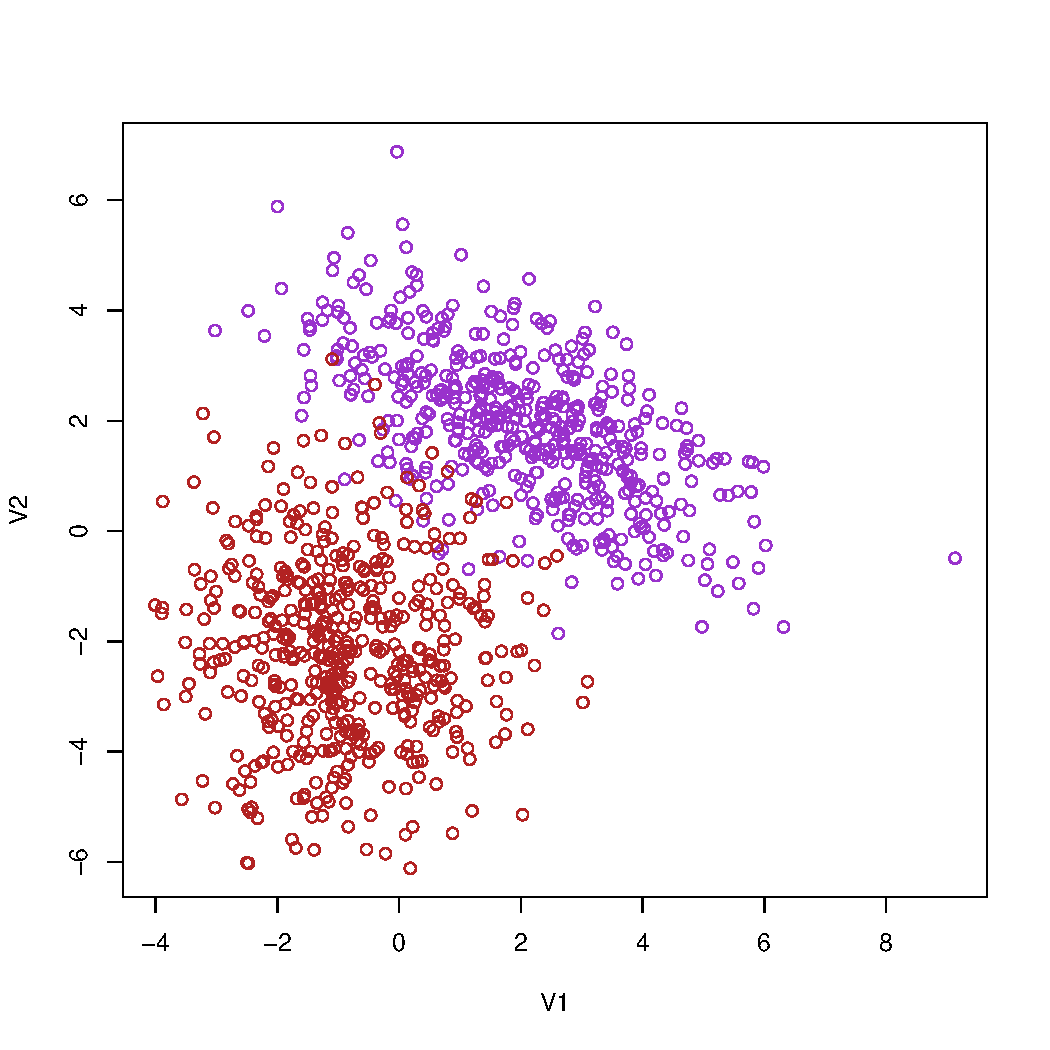
\includegraphics[width=0.35\textwidth]{synth_1_1000.pdf}
    \captionof{figure}{Jeu de données \texttt{Synth1-1000} afin d'émettre des hypothèses}
    \label{fig_synth_1_1000}
\endgroup

Pour le premier jeu de données observable ci-dessus, l'\textbf{ADQ} semble bien s'y adapter pour les raisons évoquer précédemment, les différents conditions sont respectés. Cependant, l'\textbf{ADL} ou bien le Classifieur Bayésien Naïf semblent moins bien s'adapter à la répartition des données. Effectivement, nous savons que a frontière de décision à associée à l'\texttt{ADL} est linéaire. Dans la figure \ref{fig_synth_1_1000}, nous remarquons que les données des deux classes ne peuvent pas bien se scinder selon une droite dans le plan. 
De plus, nous savons que la frontière de décision associée au \texttt{NBA} est plus adaptée si les dispersions associées aux données des différentes classes se font suivant les axes. Concernant les arbres binaires, il est plus complexe de conclure concernant l'adéquation du modèle avec le jeu de données. Toutefois, il est très probable que les résultats soient moins bons puisque cela revient à tenter de partition le plan sous forme de rectangles. Or, il semble que cela ne soit pas adapté à notre jeu de données. Si l'on souhaite une bonne précision pour ce jeu de données, il faudra une complexité très grande afin de bien représenter la limite des classes. Or, nous ne souhaitons pas avoir une telle complexité.
Finalement, la régression logistique, qu'elle soit classique ou quadratique devrait être mois bien adaptée que l'analyse discriminante car le jeu de donnée possède de très bonne caractéristique pour le modèle de l'analyse discriminante et il respecte ses contraintes.
\end{multicols}
\begin{multicols}{3} 
\begingroup
   \centering
   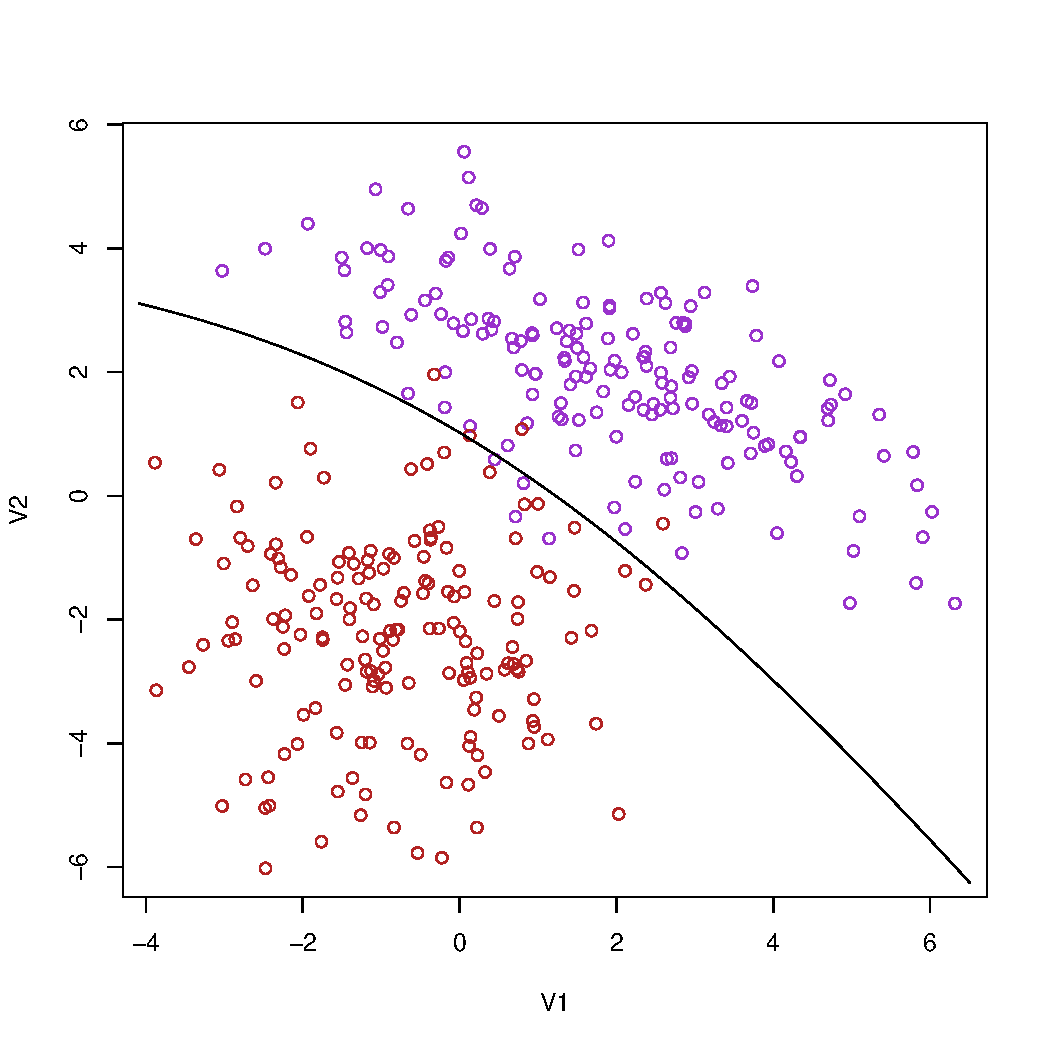
\includegraphics[width=0.28\textwidth]{synth_1_adq_1000.pdf}
    \captionof{figure}{Analyse discriminante quadratique pour le jeu de données \texttt{Synth1-1000}}
    \label{fig_synth_1_adq_1000}
\endgroup
\begingroup
   \centering
   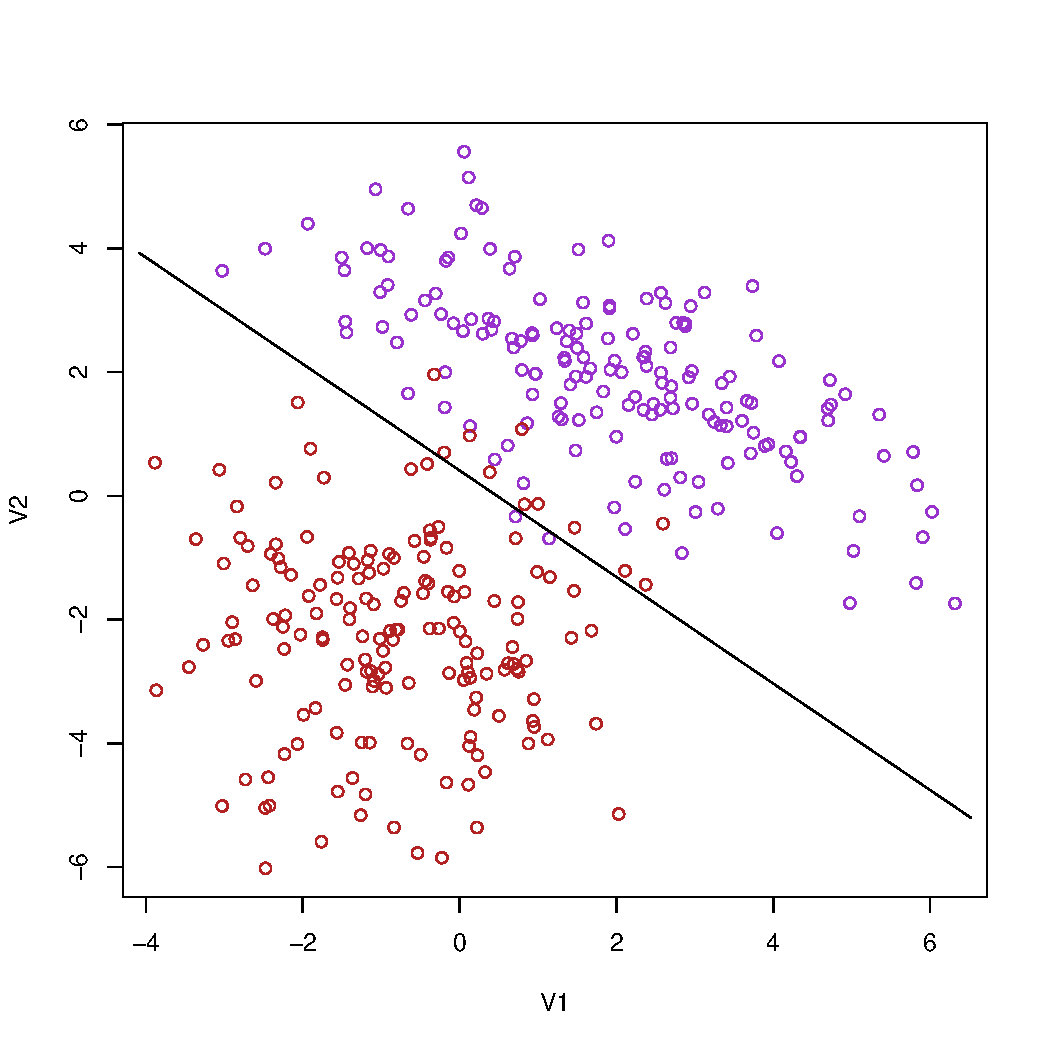
\includegraphics[width=0.28\textwidth]{synth_1_adl_1000.pdf}
    \captionof{figure}{Analyse discriminante linéaire pour le jeu de données \texttt{Synth1-1000}}
    \label{fig_synth_1_adl_1000}
\endgroup
\begingroup
   \centering
   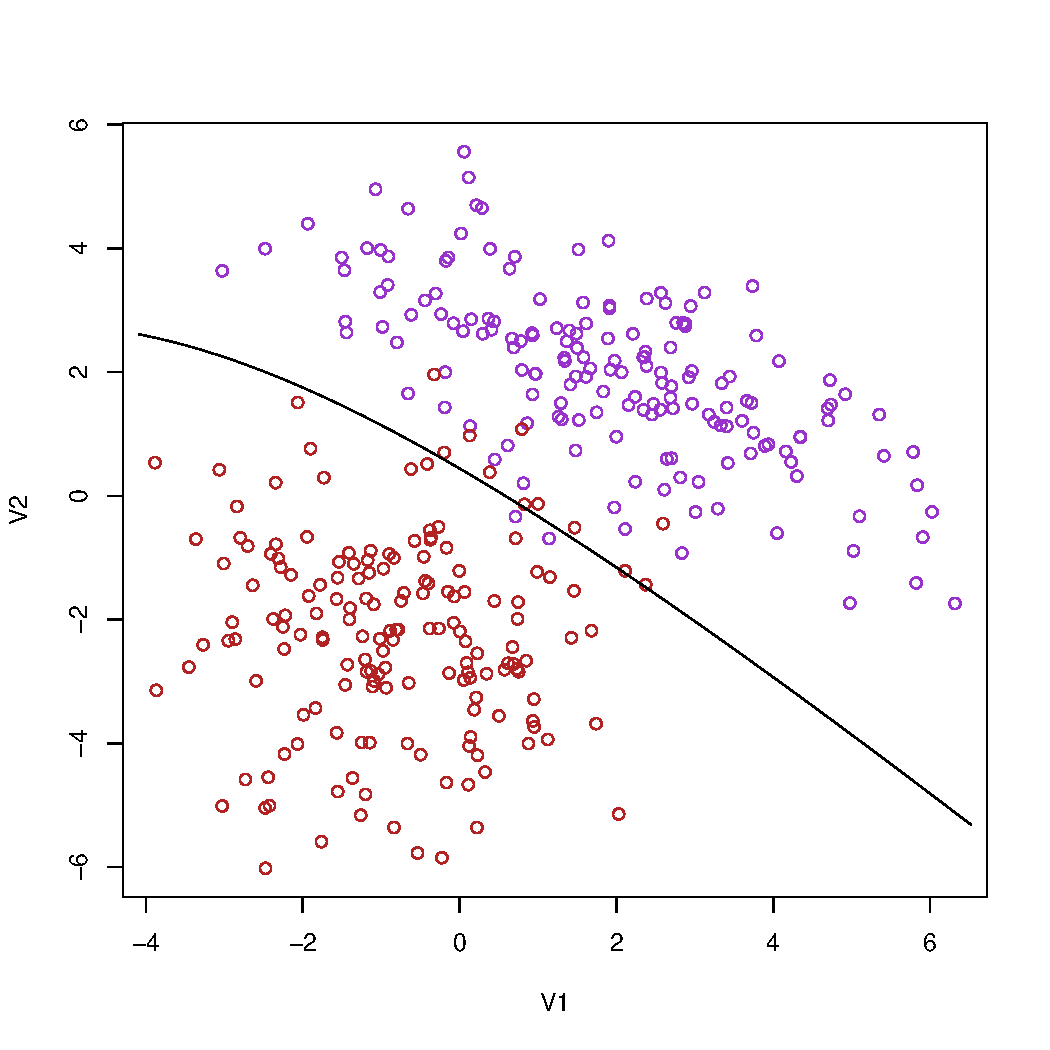
\includegraphics[width=0.28\textwidth]{synth_1_nba_1000.pdf}
    \captionof{figure}{classifieur bayésien naïf pour le jeu de données \texttt{Synth1-1000}}
    \label{fig_synth_1_nba_1000}
\endgroup
\begingroup
   \centering
   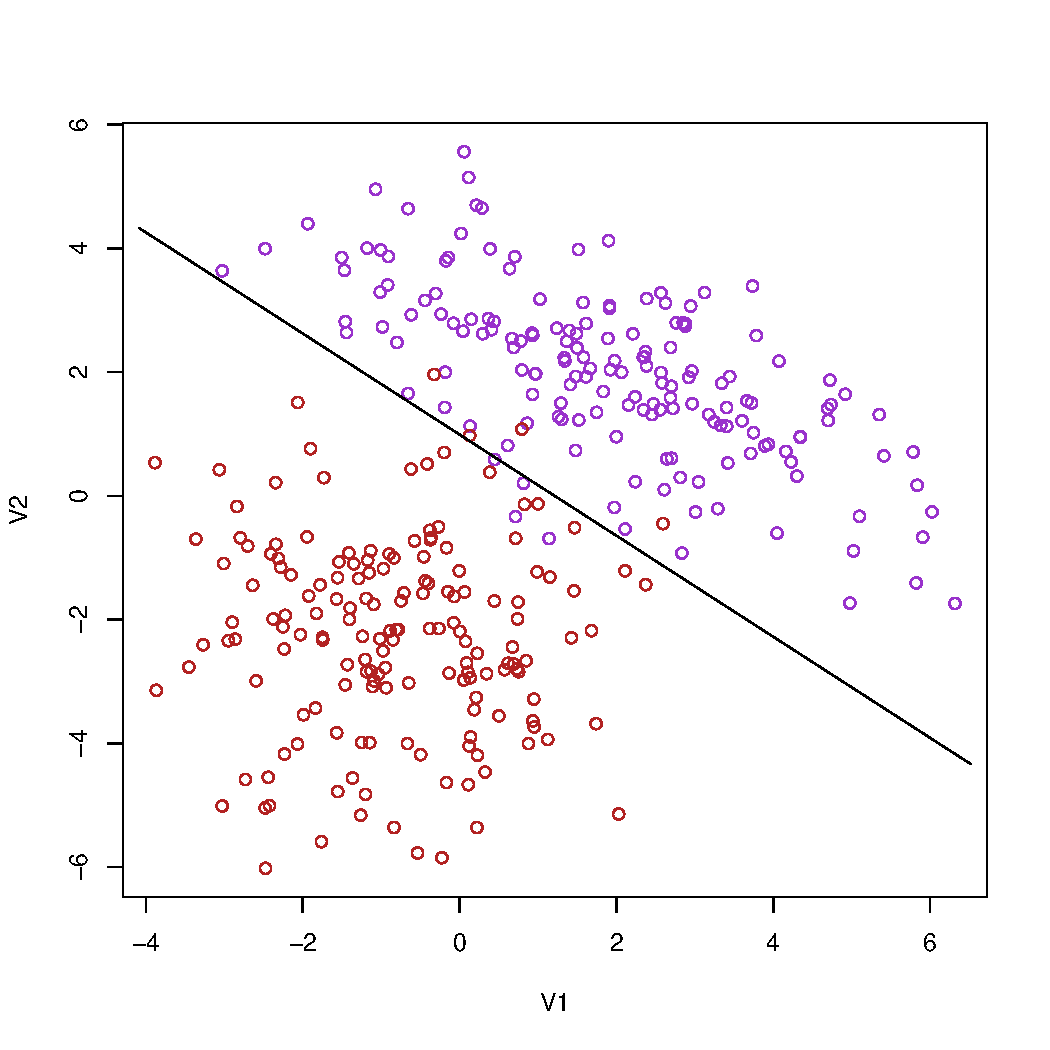
\includegraphics[width=0.28\textwidth]{synth_1_log_with_intercept_1000.pdf}
    \captionof{figure}{Régression Logistique classique avec intercept pour le jeu de données \texttt{Synth1-1000}}
    \label{fig_synth_1_log_with_intercept_1000}
\endgroup
\begingroup
   \centering
   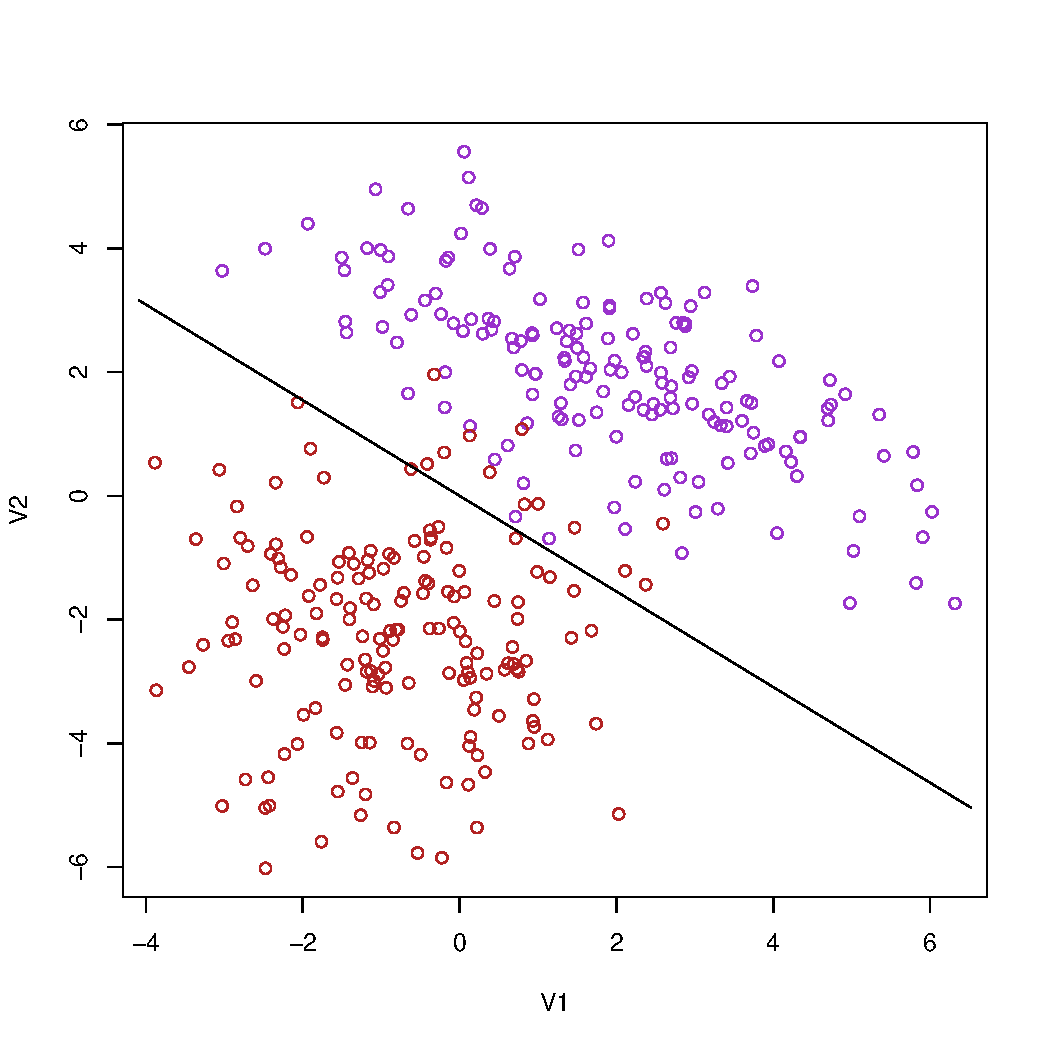
\includegraphics[width=0.28\textwidth]{synth_1_log_without_intercept_1000.pdf}
    \captionof{figure}{Régression Logistique classique sans intercept pour le jeu de données \texttt{Synth1-1000}}
    \label{fig_synth_1_log_without_intercept_1000}
\endgroup
\begingroup
   \centering
   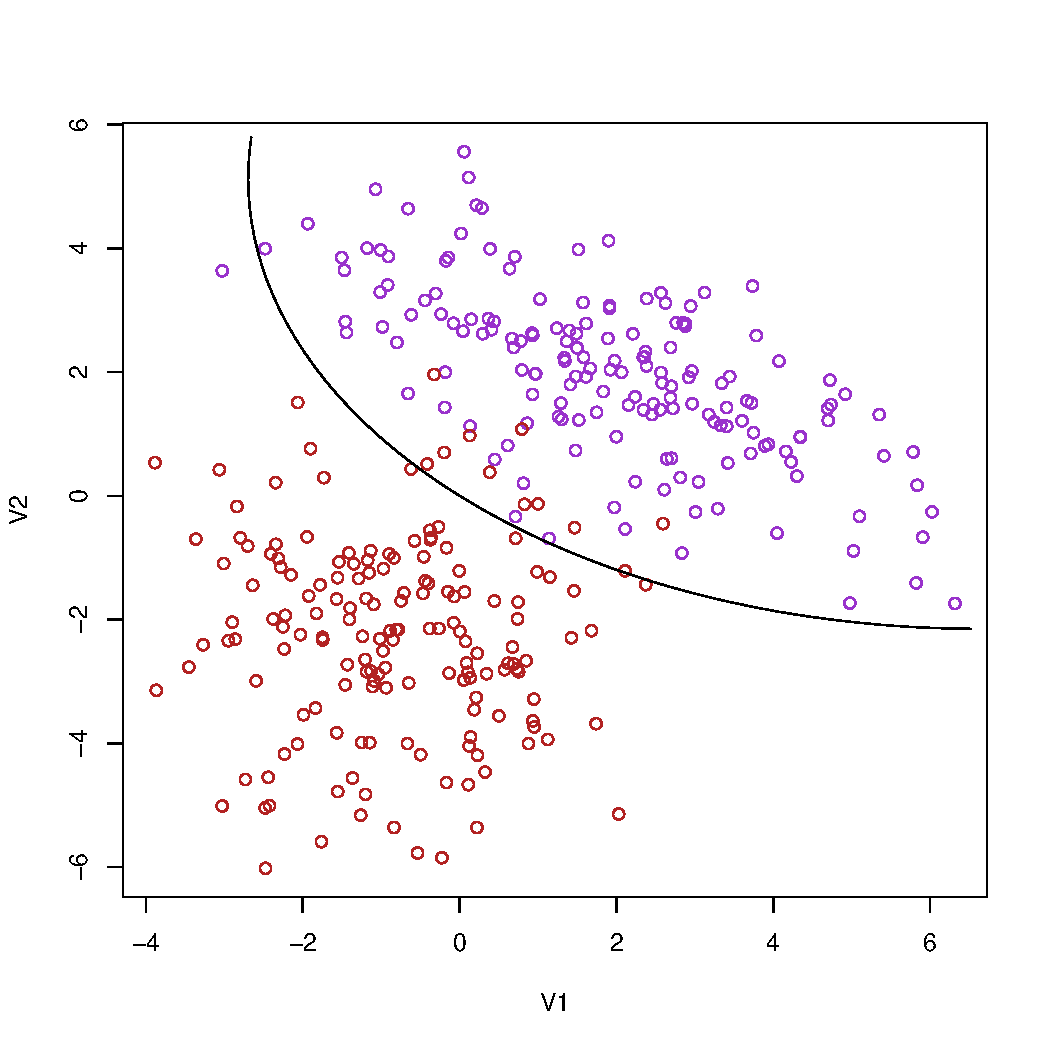
\includegraphics[width=0.28\textwidth]{synth_1_quad_log_1000.pdf}
    \captionof{figure}{Régression Logistique quadratique pour le jeu de données \texttt{Synth1-1000}}
    \label{fig_synth_1_quad_log_1000}
\endgroup
\begingroup
   \centering
   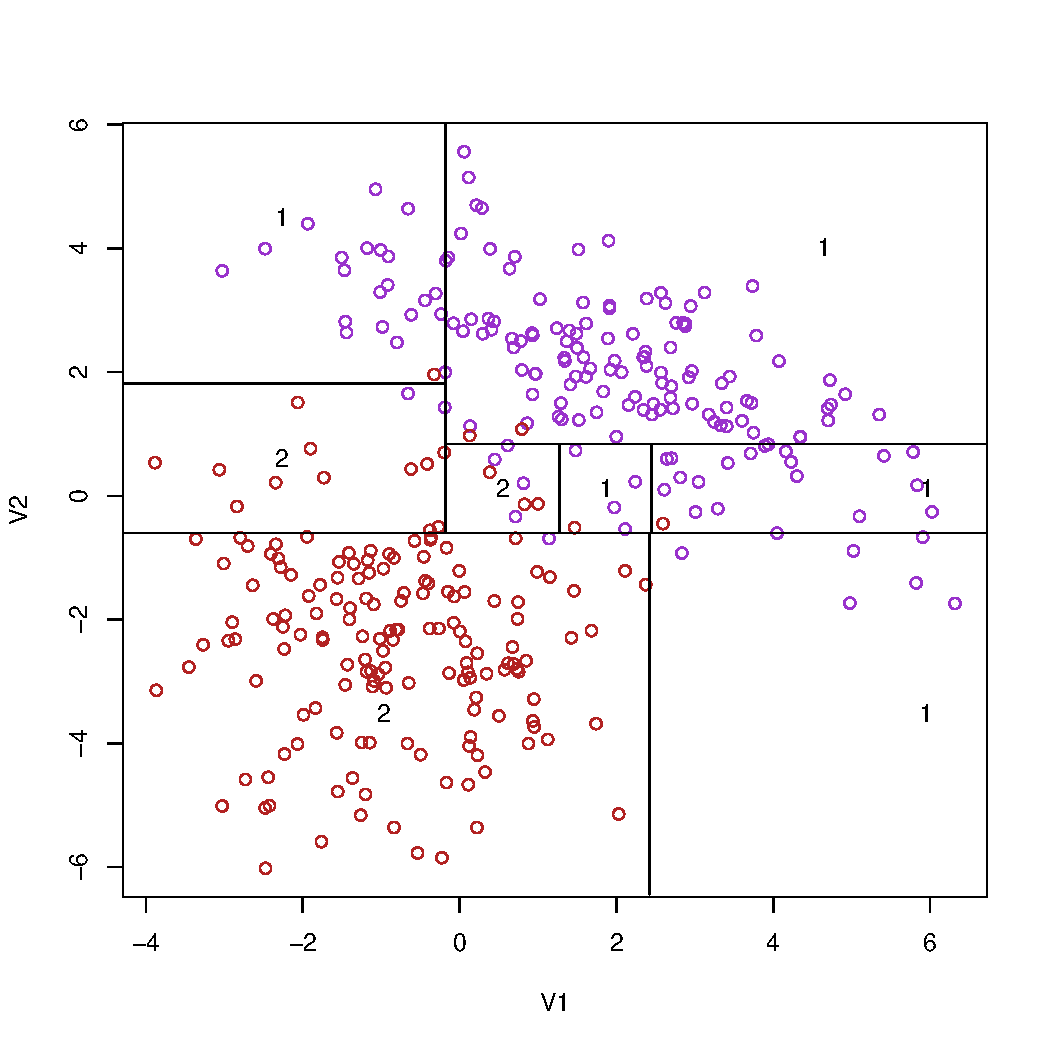
\includegraphics[width=0.28\textwidth]{synth_1_bin_partition_1000.pdf}
    \captionof{figure}{Arbre binaire pour le jeu de données \texttt{Synth1-1000}}
    \label{fig_synth_1_bin_partition_1000}
\endgroup
\begingroup
   \centering
   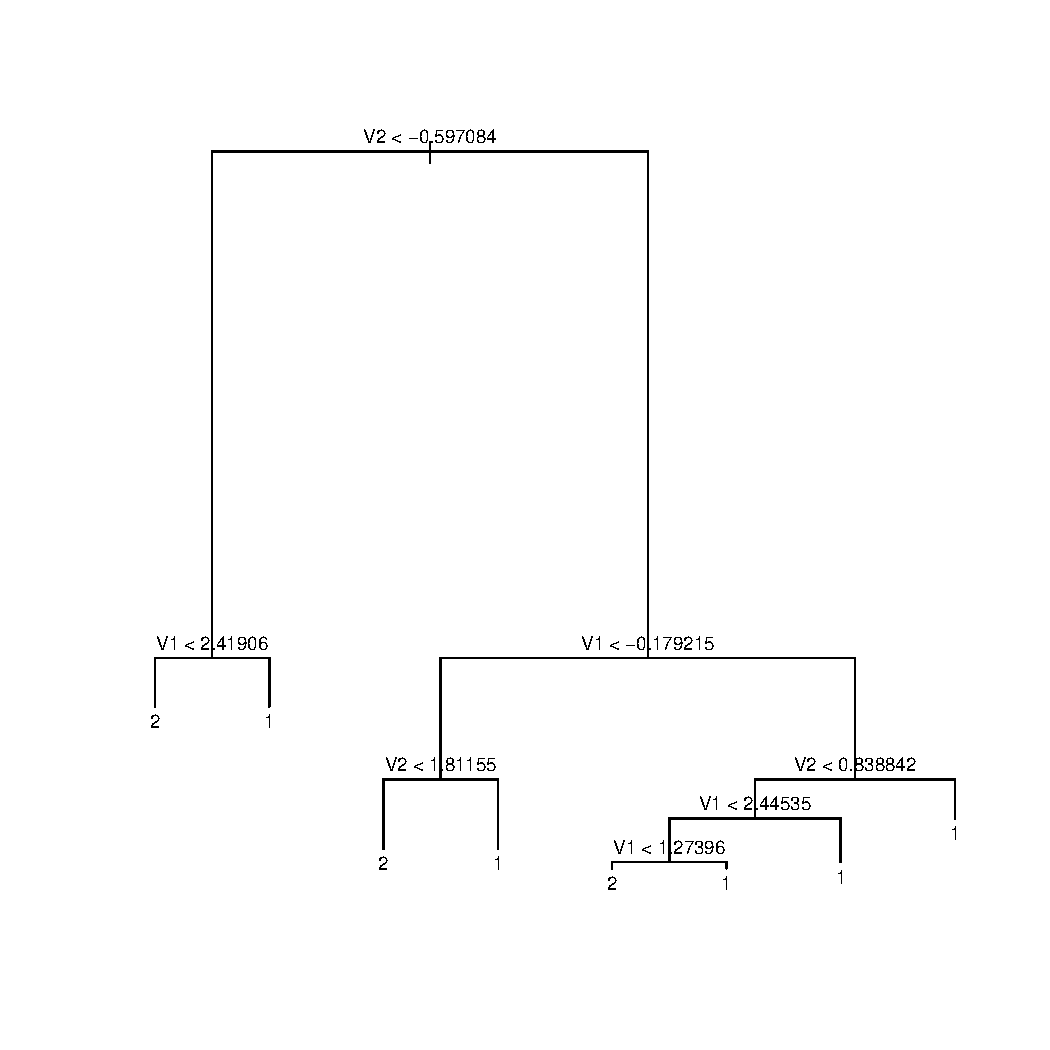
\includegraphics[width=0.28\textwidth]{synth_1_bin_tree_1000.pdf}
    \captionof{figure}{Arbre binaire obtenu pour le jeu de données \texttt{Synth1-1000}}
    \label{fig_synth_1_bin_tree_1000}
\endgroup
\end{multicols}
\begin{multicols}{2}  
\begingroup
   \centering
   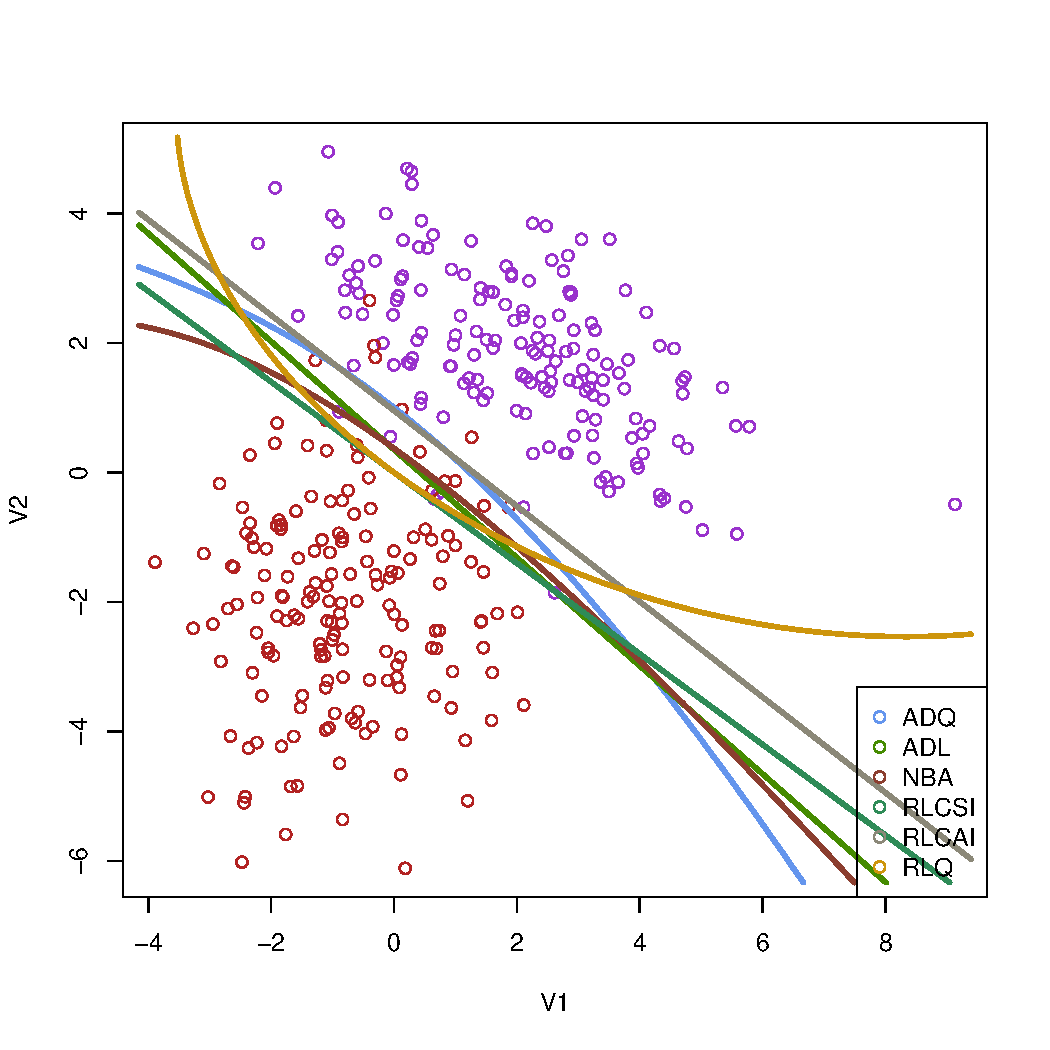
\includegraphics[width=0.5\textwidth]{synth_1_all_models.pdf}
    \captionof{figure}{Représentation des frontières de décisions des modèles pour \texttt{Synth1-1000}}
    \label{fig_synth_1_model_partition_1000}
\endgroup
Cette dernière représentation permet d'observer les frontières de décisions pour tous les modèles sauf l'arbre binaire.
Nous allons maintenant montrer les différents résultats obtenus ainsi que leurs erreurs résumé dans un tableau :

\begin{center}
\begin{tabular}{| c || c | c |}
\hline
\texttt{Synth1-1000} & $\widehat{\varepsilon}_i$  & $IC_{\varepsilon_{i}}$  \\
\hline
\hline
\texttt{ADQ} & 2.52 \% & [2.16, 2.88] \\
\hline
\texttt{ADL} & 3.54 \% & [3.14, 3.94] \\
\hline
\texttt{NBA} & 3.56 \% & [3.17, 3.95] \\
\hline
\texttt{RLCSI} & 4.13 \% & [3.72, 4.53] \\
\hline
\texttt{RLCAI} & 2.56 \% & [2.18, 2.95] \\
\hline
\texttt{RLQ} &  3.74 \% & [3.37, 4.11] \\
\hline
\texttt{BT} & 3.90 \% & [3.51, 4.30] \\
\hline
\end{tabular}\\ 
\label{table_Synth1-1000}
\end{center}

Les erreurs semblent nous indiquer que l'\textbf{ADQ} est le meilleur modèle pour ce jeu de données \textit{synth1\_1000} ! Son point négatif étant sa complexité et le besoin d'un grand nombre de données. Cela n'est pas un problème dans ce cas de figure mais il faut garder à l'esprit ses inconvénients. La \textbf{régression logistique avec intercept} fait aussi office de sérieux candidat, les autres modèles présentent des performances acceptables mais très en dessous de celle de l'\textbf{ADQ}.

\subsubsection{Synth2-1000}
\label{subsubsec_Synth2_1000}

\begingroup
   \centering
   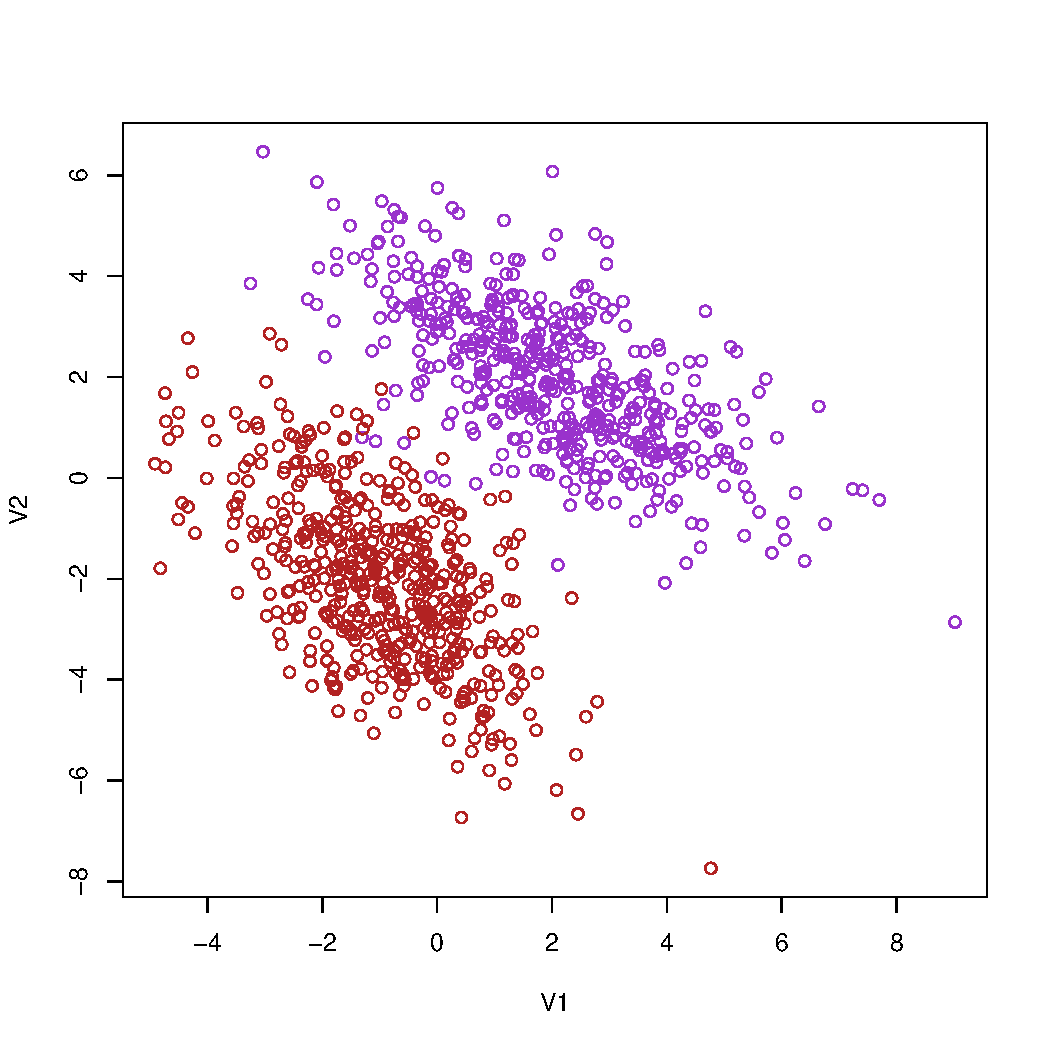
\includegraphics[width=0.3\textwidth]{synth_2_1000.pdf}
    \captionof{figure}{Jeu de données \texttt{Synth2-1000} afin d'émettre des hypothèses}
    \label{fig_synth_2_1000}
\endgroup

Nous émettons de nouvelles hypothèses à partir de ce second jeu de données \textit{synth2\_1000}. Dans ce cas, il nous semble que l'ADQ sera toujours aussi efficient mais l'ADL semble être un très bon candidat dû à la distribution des valeurs comme cela peut s'observer sur le graphique, la création d'une frontière linéaire entre les 2 classes semblent aisées car celle-ci ne se mélangent peu et suivent une même orientations. Les hypothèses concernant les autres jeu sont assez proches de celle émise pour le jeu précédent, nous ne les détaillerons pas.

Voici le tableau récapitulatif des erreurs : 
\begin{center}
\begin{tabular}{| c || c | c |}
\hline
\texttt{Synth2-1000} & $\widehat{\varepsilon}_i$  & $IC_{\varepsilon_{i}}$  \\
\hline
\hline
\texttt{ADQ} & 0.97 \% & [0.78, 1.16] \\
\hline
\texttt{ADL} & 1.06 \% & [0.92, 1.21] \\
\hline
\texttt{NBA} & 1.60 \% & [1.40, 1.80] \\
\hline
\texttt{RLCSI} & 1.16 \% & [0.91, 1.42] \\
\hline
\texttt{RLCAI} & 1.15 \% & [0.99, 1.31] \\
\hline
\texttt{RLQ} &  1.14 \% & [0.98, 1.29] \\
\hline
\texttt{BT} & 1.68 \% & [1.38, 1.97] \\
\hline
\end{tabular}\\
\label{table_Synth2-1000}
\end{center}
Comme émit en hypothèse, les modèles \textbf{ADQ} et \textbf{ADL} semble être les plus adapté avec aussi \textbf{la régression logistique sans intercept}.
L'ADQ possède de légère meilleur performance mais sa complexité nécessite beaucoup plus de données. De plus, l'ADL est plus robuste.
Ici, nous avons donc le choix de l'ADQ qui est un peu mieux mais qui dépend vraiment du jeu de données et notamment de sa taille sinon l'ADL, plus robuste, est bon modèle aussi. On peut voir graphiquement que les courbes sont d'ailleurs très similaires.

\newpage

Voici le graphique avec les frontières de décisions des modèles (hormis l'arbre binaire) pour ce jeu de données :

\begingroup
   \centering
   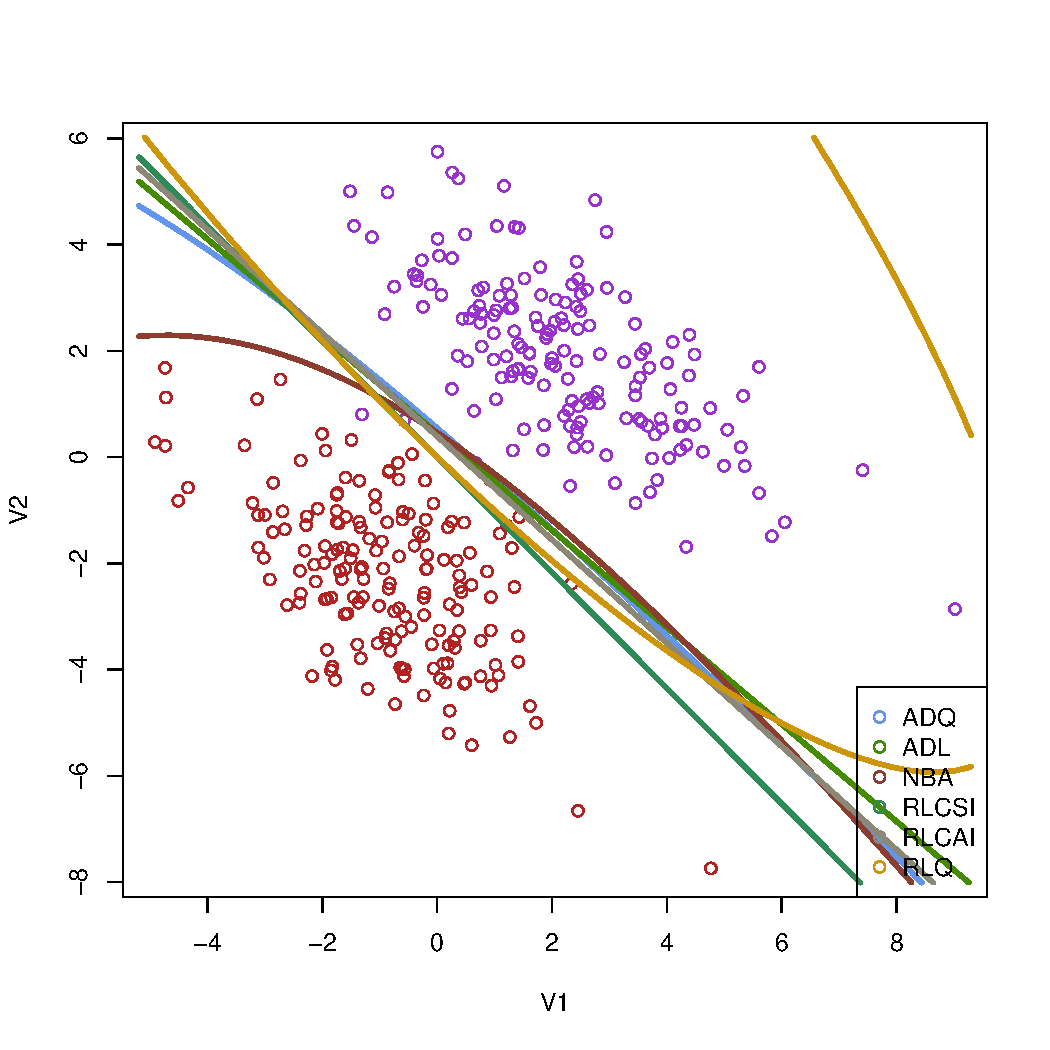
\includegraphics[width=0.5\textwidth]{synth_2_all_models.pdf}
    \captionof{figure}{Représentation des frontières de décisions des modèles pour \texttt{Synth2-1000}}
    \label{fig_synth_2_adq_1000}
\endgroup

\subsubsection{Synth3-1000}
\label{subsubsec_Synth3_1000}

\begingroup
   \centering
   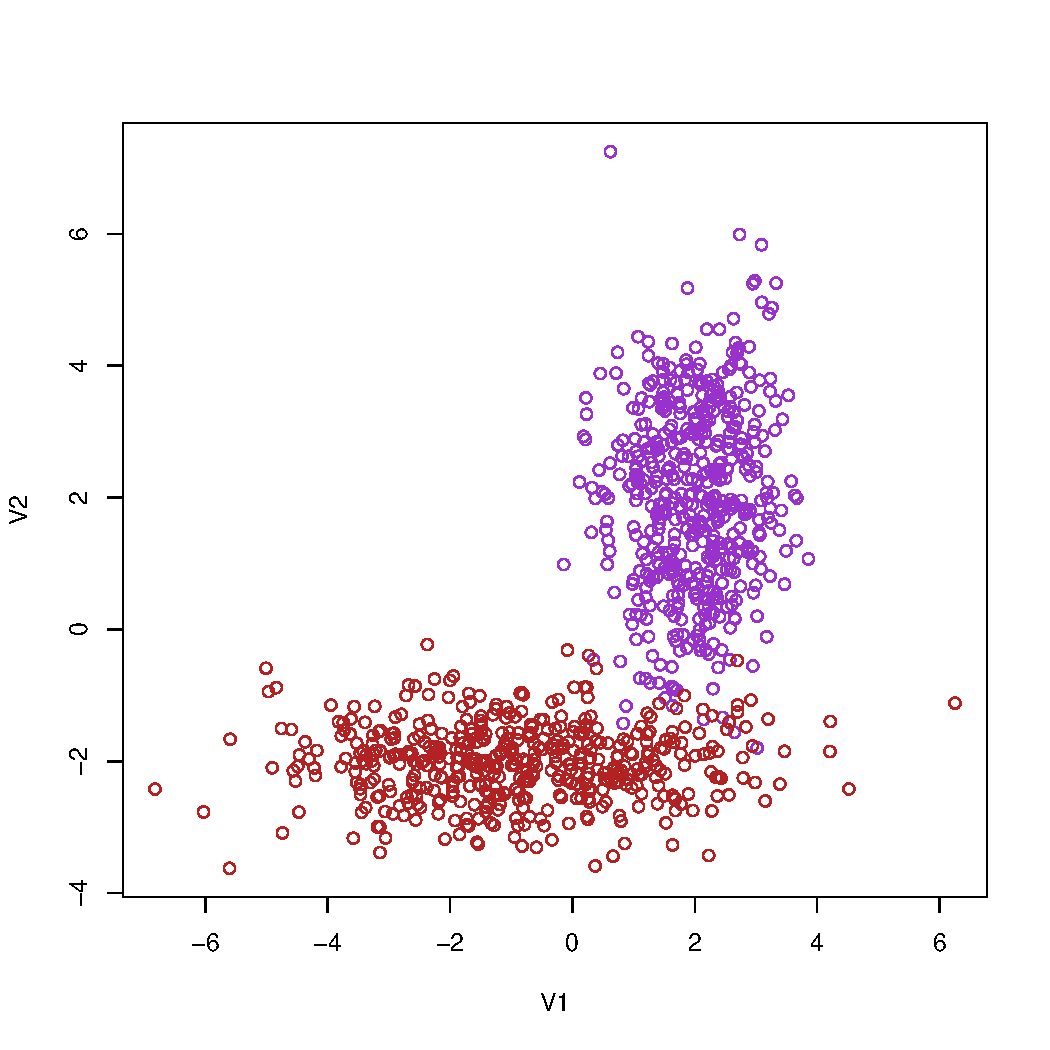
\includegraphics[width=0.4\textwidth]{synth_3_1000.pdf}
    \captionof{figure}{Jeu de données \texttt{Synth3-1000} afin d'émettre des hypothèses}
    \label{fig_synth_3_1000}
\endgroup

Voici notre troisième et dernier jeu de données synthétisée, \textit{synth3\_1000}. Au vu de la distribution des 2 classes qui semble chacune suivre un axe (la classe violette suit les ordonnées alors que la rouge suit les abscisses), le classifieur bayésien naïf en plus de l'ADQ nous semble être un choix correct cette fois-ci.

Voici le tableau récapitulatif des erreurs :
\begin{center}
\begin{tabular}{| c || c | c |}
\hline
\texttt{Synth3-1000} & $\widehat{\varepsilon}_i$  & $IC_{\varepsilon_{i}}$  \\
\hline
\hline
\texttt{ADQ} & 1.25 \% & [1.04, 1.45] \\
\hline
\texttt{ADL} & 2.43 \% & [2.14, 2.72] \\
\hline
\texttt{NBA} & 1.35 \% & [1.14, 1.56] \\
\hline
\texttt{RLCSI} & 2.55 \% & [2.30, 2.81] \\
\hline
\texttt{RLCAI} & 1.80 \% & [1.52, 2.09] \\
\hline
\texttt{RLQ} &  1.41 \% & [1.19, 1.63] \\
\hline
\texttt{BT} & 1.80 \% & [1.58, 2.03] \\
\hline
\end{tabular}\\ 
\label{able_Synth3-1000}
\end{center}
Cette fois il semblerait que l'\textbf{ADQ}, le \textbf{NBA} et la \textbf{régression logistique quadratique} soit les modèles avec les meilleurs performances. Cependant au vu de la complexité de mettre en place le NBA, son choix final n'est sûrement pas le plus pertinent malgré ses performances. L'ADQ semble une nouvelle fois le plus appropriée.
On pourra remarquer éventuellement la taille de l'intervalle de confiance pour l'arbre binaire qui est logiquement plus élevée.

Voici les graphiques illustrant ces résultats (hormis l'arbre binaire) :

\begingroup
   \centering
   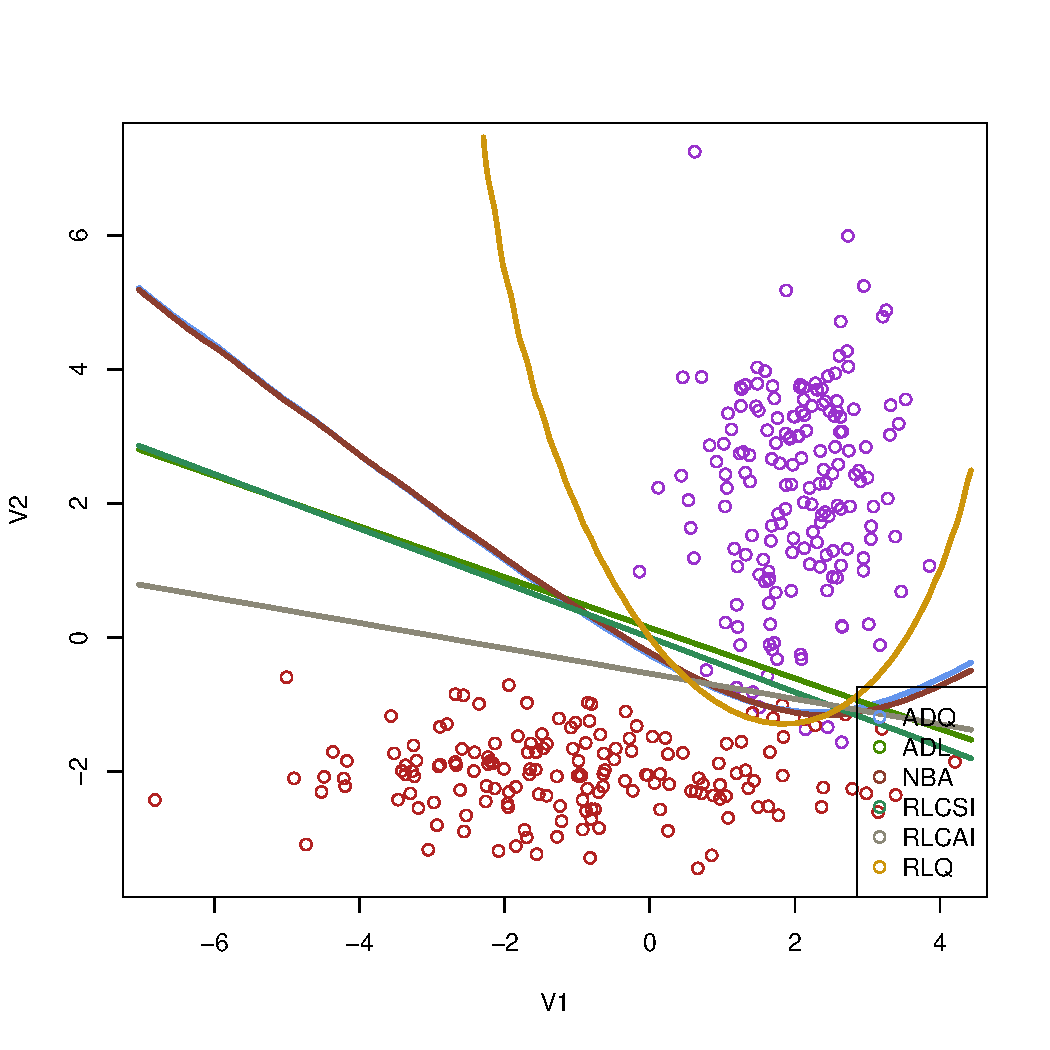
\includegraphics[width=0.5\textwidth]{synth_3_all_models.pdf}
    \captionof{figure}{Représentation des frontières de décisions des modèles pour \texttt{Synth3-1000}}
\endgroup
\newpage
\subsection{Test sur données réelles}
\label{subsec_Testsurdonneesreelles}

\subsubsection{Données « Pima »}
\label{subsubsec_donneespima}
Dans cette sous-sous-section, nous avons appliqué les trois modèles d'analyse discriminante, les deux modèles de régression logistique et les arbres de décision à la prédiction du diabète chez les individus d'une population d'amérindiens. Les données étaient présentes dans le fichier \texttt{Pima.csv} sur le site de l'UV. Ce dernier contient $n = 532$ individus décrits chacun par $p = 7$ variables explicatives. 

Afin d'apprendre et pouvoir faire des prédictions à partir de ce dernier, nous avons utiliser le même protocole expérimental que pour les tests sur les données simulées (sous-section \ref{subsec_testsurdonneessimulees}) en répétant cette fois-ci l'expérience $N = 100$ fois. Ainsi, pour chacun des modèles, nous avons calculé les estimations ponctuelles  $\widehat{\varepsilon}_i = \bar{\varepsilon}_i$ des taux d’erreurs $\varepsilon_i$ de test et les intervalles de confiance bilatéraux $IC_{\varepsilon_{i}}$ pour les mêmes paramètres au niveau de confiance $1 - \alpha,$ où $\alpha = 0.05.$ Nous noterons que l'approximation sera probablement de bonne qualité puisque $N \geq 30.$

Ci-dessous, figurent les estimations pour les différents modèles.
\begin{center}
\begin{tabular}{| c || c | c |}
\hline
\texttt{Pima.csv} & $\widehat{\varepsilon}_i$ \% & $IC_{\varepsilon_{i}}$ \% \\
\hline
\hline
\texttt{ADQ} & 23.84 & [23.30, 24.37] \\
\hline
\texttt{ADL} & 21.69 & [21.16, 22.23] \\
\hline
\texttt{NBA} & 23.30 & [22.73, 23.87] \\
\hline
\texttt{RLCSI} & 28.46 & [27.96, 28.97] \\
\hline
\texttt{RLCAI} & 21.44 & [20.90, 21.98] \\
\hline
\texttt{RLQ} &  24.54 & [24.04, 25.03] \\
\hline
\texttt{BT} & 23.88 & [23.24, 24.52] \\
\hline
\end{tabular}\\ 
\label{table_Pima}
\end{center}

Tout d'abord, nous constatons que les estimations  $\widehat{\varepsilon}_i$  des taux d'erreurs de test $\varepsilon_i$ sont toutes supérieures à $20 \%.$ Cela semble cohérent puisque les taux d'erreur de prédiction du diabète ont généralement ces ordres de grandeur. 

Nous constatons que l'estimation du taux d'erreur associée à la  \texttt{RLCAI} est plus faible que celle associée à la \texttt{RLCSI}. Cela est tout à fait cohérent puisque le jeu de données est relativement grand $p = 7$ variables descriptives $n = 532$ individus. Or, nous savons que la \texttt{RLCAI} apprend un paramètre de plus que la 
\texttt{RLCSI}. Ainsi, la taille de la population couplée à ce paramètre d'apprentissage supplémentaire permettent d'obtenir de meilleurs résultats.

Cependant, on constate également que l'estimation du taux d'erreur associée à la \texttt{RLQ} est supérieure à celle associée à la \texttt{RLCAI}. Certes, on apprend plus de paramètres avec la \texttt{RLQ}. Toutefois, ce nombre plus élevé de paramètres à apprendre requiert nécessairement un jeu de données plus imposant pour que les paramètres correspondent à l'existant. Ainsi, il semblerait que le jeu de données ne soit pas assez conséquent pour que les résultats obtenus via la \texttt{RLQ} soient meilleures que ceux obtenus via la \texttt{RLCAI}. 

Par ailleurs, on constate également que l'hypothèse que le vecteur caractéristique $X$ suit, conditionnellement à chaque classe $\omega_k$, une loi normale multidimensionnelle d'espérance $\mu_k$ et de variance $\Sigma_k$ n'est pas mauvaise puisque les estimations des taux d'erreur obtenues via les analyses discriminantes sont du même ordre de grandeur que celles obtenues via les régressions logistiques. 

De plus, on constate que l'estimation du taux d'erreur associée à l'\texttt{ADQ} est supérieure à celle de l'\texttt{ADL}. A l'instar de la \texttt{RLQ}, cela peut s'expliquer par le fait que le nombre plus élevé de paramètres à apprendre requiert un jeu de données de taille plus imposante pour que les paramètres à apprendre correspondent à l'existant. Ainsi, il semblerait à nouveau que le jeu de données ne soit pas assez conséquent pour que les résultats obtenus via l'\texttt{ADQ} soient meilleurs que ceux obtenus via l'\texttt{ADL}. 

De plus, on constate que l'estimation du taux d'erreur associée au \texttt{NBA} est supérieure à celle de l'\texttt{ADL}. Il semblerait que l'hypothèse d'indépendance des variables $X_j$ conditionnellement à $Z$ ne soit pas adaptée. Autrement dit, il semblerait qu'il y a corrélation entre certaines des variables. Cela suffit à expliquer les résultats de moins bonne qualité obtenus. 

Enfin, l'estimation du taux d'erreur associée au \texttt{BT} est plus élevée que celle associée à l'\texttt{ADL} et que celle associée à la \texttt{RLCAI}. En fonction du contexte et des besoins du client, l'usage de la \texttt{BT} peut se révéler être particulièrement utile. Effectivement, cela permet d'attribuer des probabilités a posteriori à chacune des feuilles de l'arbre. A titre d'exemple, cela peut-être utilisée à des fins de prise de décision. On peut décider de faire effectuer des tests plus onéreux à un patient dont la probabilité d'être diabétique dépasse un certain seuil. De même, l'interprétabilité de cette méthode est un de ses autres avantages. Cette méthode peut également permettre de justifier une prise de décision. La justification est particulièrement simple et compréhensible grâce aux variables explicatives du jeu de données. A titre d'exemple (figure \ref{pima_bcw_tree}), si l'individu a un taux de glucose inférieur à $127.5$, il a de fortes chances de ne pas être diabétique. S'il présente un taux de glucose supérieur à $157.5$, il a de fortes de chances de l'être.

\begingroup
   \centering
   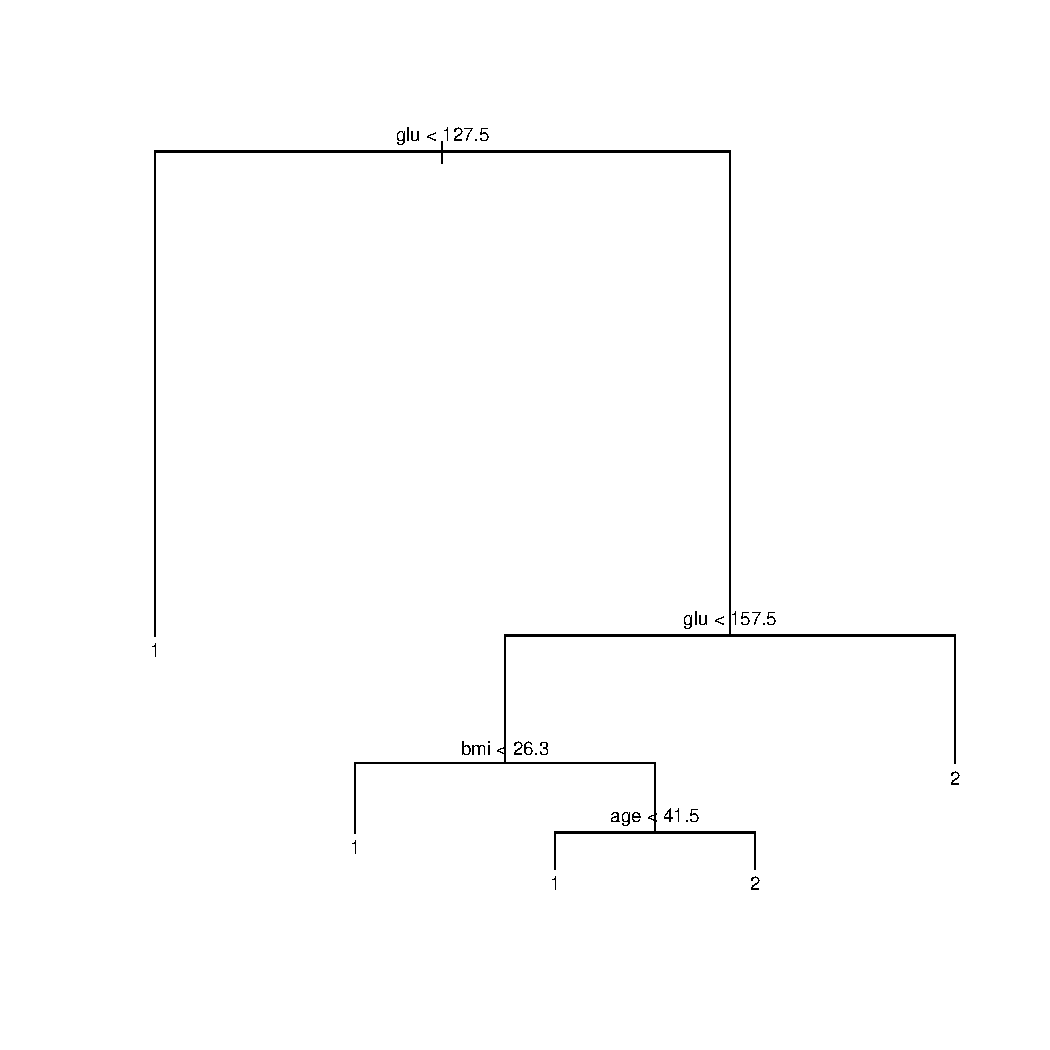
\includegraphics[width=0.35\textwidth]{pima_bin_tree.pdf}
    \captionof{figure}{Arbre de décision obtenue à l'issue d'une séparation aléatoire de $\frac{2}{3}$ du jeu de données \texttt{Pima.csv}}
    \label{pima_bcw_tree}
\endgroup

\subsubsection{Données "breast cancer Wisconsin"}
\label{subsubsec_donneesbcw}
Dans cette sous-sous-section, nous nous sommes intéressés à un problème de prédiction du niveau de gravité d'une tumeur à partir de descripteurs physiologiques. Les données figuraient dans le fichier \texttt{bcw.csv} sur le site de l'UV. Ce dernier contient $n = 683$ individus décrits chacun par $p = 9$ variables explicatives. 

A l'instar de la sous-sous-section \ref{subsubsec_donneespima}, nous avons répété l'expérience (séparation, apprentissage et évaluation des performances) $N = 100$ fois. De plus, nous avons évalué les taux moyens d'erreur de test pour les trois modèles d'analyse discriminante, la régression logistique classique (il était demandé dans l'énoncé de ne pas utiliser la régression logistique quadratique) et les arbres de décision.

Ci-dessous, figurent les estimations pour les différents modèles. 

\begin{center}
\begin{tabular}{| c || c | c |}
\hline
\texttt{Pima.csv} & $\widehat{\varepsilon}_i$ \% & $IC_{\varepsilon_{i}}$ \% \\
\hline
\hline
\texttt{ADQ} & 5.07 & [4.83, 5.31] \\
\hline
\texttt{ADL} & 4.55 & [4.34, 4.76] \\
\hline
\texttt{NBA} & 3.87 & [3.67, 4.07] \\
\hline
\texttt{RLCSI} & 15.77 & [15.39, 16.14] \\
\hline
\texttt{RLCAI} & 4.12 & [3.91, 4.34] \\
\hline
\texttt{BT} & 5.64 & [5.35, 5.93] \\
\hline
\end{tabular}\\ 
\end{center}

Tout d'abord, nous constatons que les estimations  $\widehat{\varepsilon}_i$  des taux d'erreurs de test $\varepsilon_i$ sont toutes supérieurs à $6 \%$ sauf celle de \texttt{RLCSI}. Le fait que la quasi-totalité des modèles présente des estimations de taux d'erreur du même ordre semble confirmer la cohérence de nos résultats. 

Tout d'abord, nous constatons que l'estimation du taux d'erreur associé à la \texttt{RLCAI} est beaucoup plus faible que celui associé à la \texttt{RLCSI}. A nouveau cela est parfaitement cohérent puisque le jeu de données est relativement grand $p = 9$ variables descriptives $n = 683$ individus. Or, nous savons que la \texttt{RLCAI} apprend un paramètre de plus que la \texttt{RLCSI}. Le taille de la population couplée à ce paramètre supplémentaire d'apprentissage justifie l'obtention de meilleurs résultats.

Par ailleurs, on constate que l'hypothèse que le vecteur caractéristique $X$ suit, conditionnellement à chaque classe $\omega_k$, une loi normale multidimensionnelle d'espérance $\mu_k$ et de variance $\Sigma_k$ n'est pas mauvaise puisque les estimations des taux d'erreur obtenues via les analyses discriminantes sont du même ordre de grandeur que celle obtenue via la \texttt{RLCAI}. 

De plus, on constate que l'estimation du taux d'erreur associée à l'\texttt{ADQ} est supérieure à celle de l'\texttt{ADL}. Cela s'explique à nouveau par le fait que le nombre plus élevé de paramètres à apprendre requiert un jeu de données plus imposant pour que les paramètres appris soient pertinents. Ainsi, il semblerait que le jeu de données ne soit pas assez conséquent pour que les résultats obtenus via l'\texttt{ADQ} soient meilleurs que ceux obtenus via l'\texttt{ADL}. 

De plus, on constate que l'estimation du taux d'erreur associé au \texttt{NBA} est inférieure à celle de l'\texttt{ADL}. Il semblerait que l'hypothèse d'indépendance des variables $X_j$ conditionnellement à $Z$ soit adaptée. Autrement dit, il semblerait qu'il n'y a pas ou peu de corrélation entre les différentes variables. Cela justifie les meilleurs résultats obtenus. 

Enfin, l'estimation du taux d'erreur associée au \texttt{BT} est plus élevée que celle associée à la \texttt{NBA} et que celle associée à la \texttt{RLCAI}. A nouveau, le choix de ce modèle dépendra du contexte d'utilisation de ce dernier. Effectivement, si les clients désirent obtenir des probabilités a posteriori associées à la situation de l'individu, l'usage de ce modèle peut s'avérer pertinent. De même, si chaque proposition d'action doit faire l'objet d'une justification particulièrement précise (cela semble être le cas pour ce jeu de données), ce modèle est à nouveau particulièrement adapté. Cela se démontre assez trivialement à l'aide de la figure \ref{fig_bcw_tree}

\begingroup
   \centering
   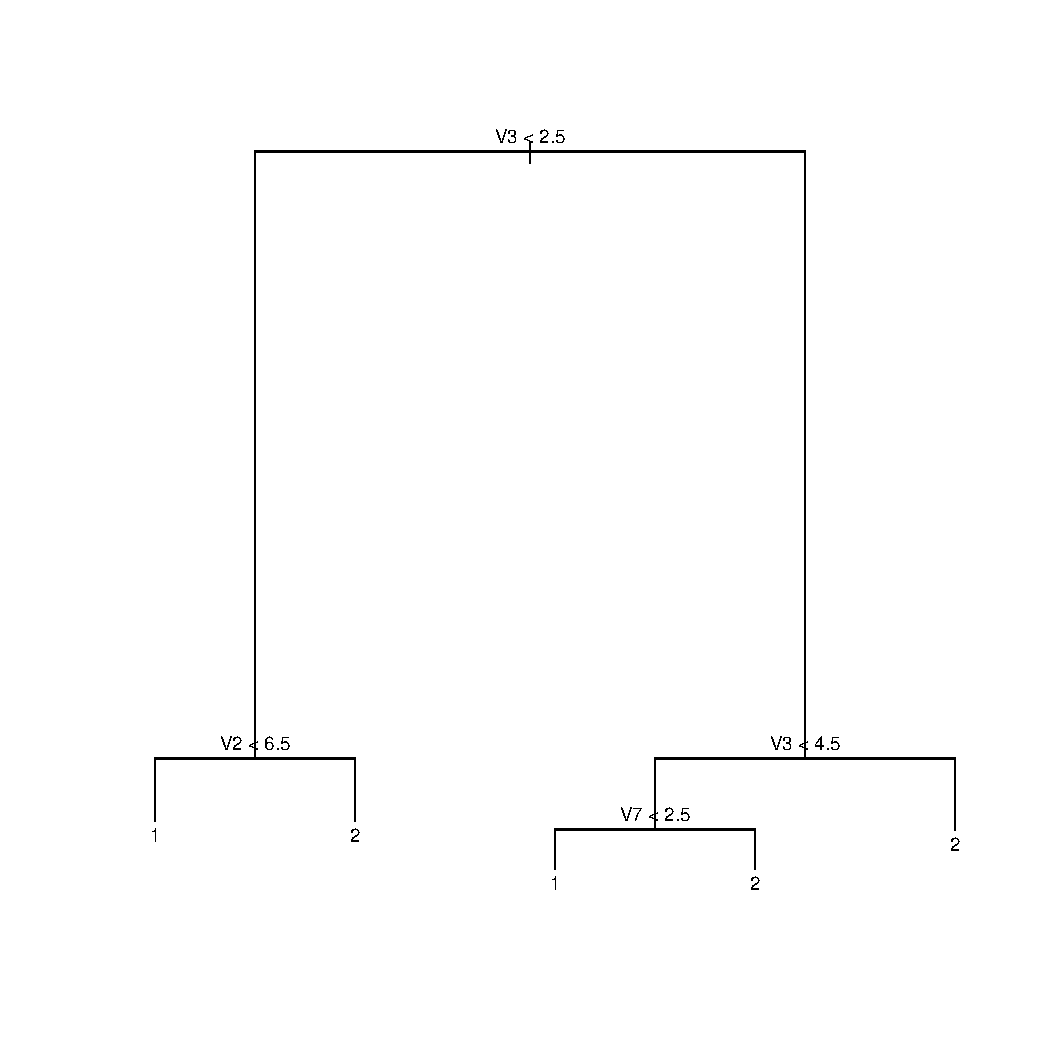
\includegraphics[width=0.35\textwidth]{bcw_bin_tree.pdf}
    \captionof{figure}{Arbre de décision obtenue à l'issue d'une séparation aléatoire de $\frac{2}{3}$ du jeu de données \texttt{bcw.csv}}
    \label{fig_bcw_tree}
\endgroup

\section{Challenge : données "Spam"}
\label{sec_challenge}
Dans cette section, nous considérons un problème de détection de spams à partir d'indicateurs calculés sur des messages électroniques. Les données figuraient dans le fichier \texttt{spam.csv} sur le site de l'UV. Le jeu de données contient $n = 4601$ individus décrits chacun par $p = 57$ variables explicatives.

A l'instar des sous-sous-sections \ref{subsubsec_donneespima} et \ref{subsubsec_donneesbcw}, nous avions pour ambition de répéter l'expérience (séparation, apprentissage et évaluation des performances) $N$ fois avant d'évaluer les taux moyens d'erreur de test pour les trois modèles d'analyse discriminante, la régression logistique classique, la régression logistique quadratique et les arbres de décision.

Toutefois, étant donné la taille du jeu de données, il était difficile de faire ces calculs pour $N \geq 30$ et donc d'obtenir de bons intervalles de confiance pour ces estimations. Par ailleurs, parmi les $7$ modèles utilisés dans ce présent rapport, il était presque sûr que certains d'entre eux ne seraient pas adaptés à notre jeu de données. En nous basant sur ce constat, nous avons choisi de suivre une stratégie particulière : nous avons décidé de commencer par discriminer les modèles inadaptés. Évidemment, étant donné les coûts en calcul particulièrement importants, il était dommage de travailler directement sur le jeu de données pour procéder à cette sélection.

Ainsi, nous avons décidé d'effectuer une ACP : les pourcentages d'inertie expliquée par les sous-espaces principaux sont consultables dans la figure \ref{fig_scree_plot_spam}.

\begingroup
   \centering
   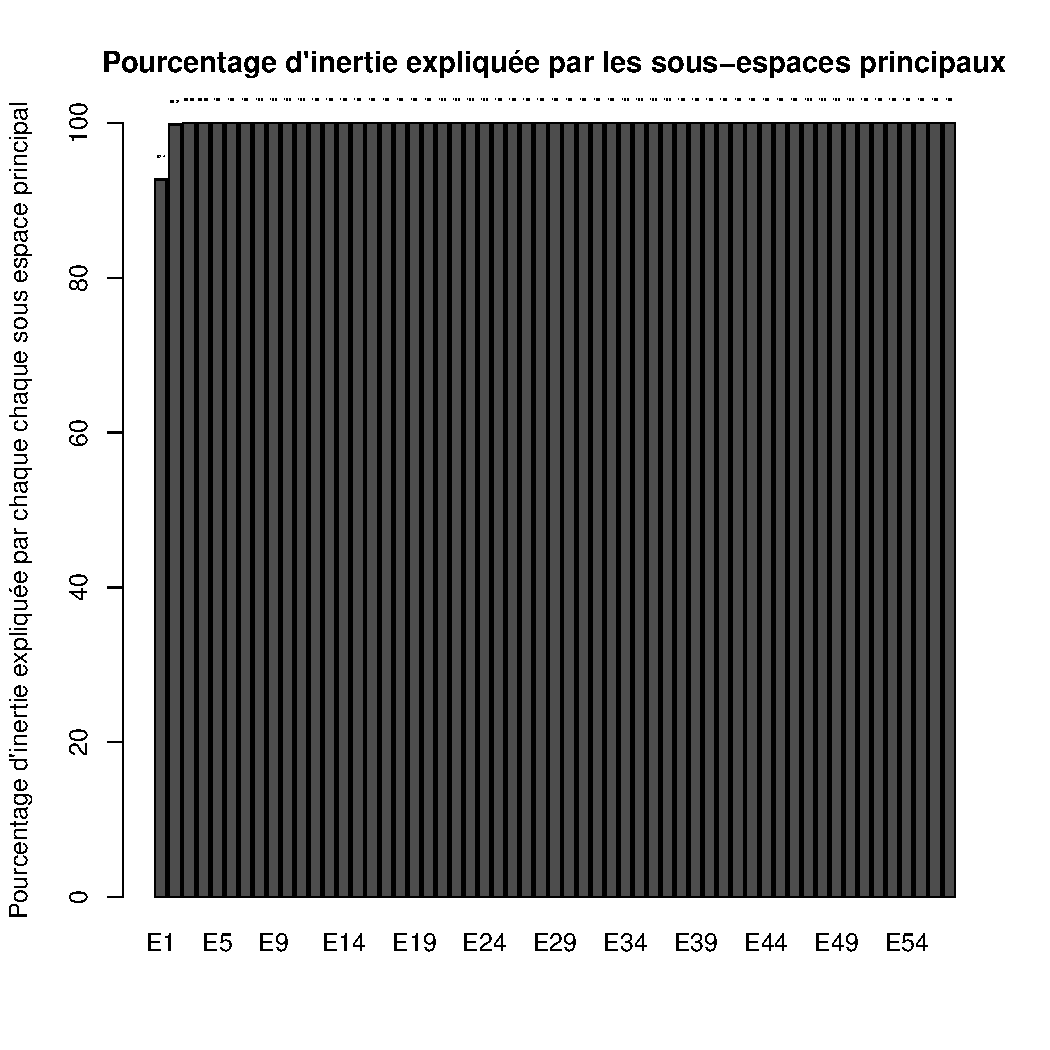
\includegraphics[width=0.35\textwidth]{fct_spam_batons_valeurs_propres_cumm.pdf}
    \captionof{figure}{Pourcentages d'inertie expliquée par les sous-espaces principaux (\texttt{spam.csv})}
    \label{fig_scree_plot_spam}
\endgroup

Dans la figure \ref{fig_scree_plot_spam}, nous constatons que le pourcentage d'inertie expliquée par le sous espace vectoriel $E_1$ est $92.7 \geq 80$. Toutefois, afin que notre sélection soit pertinente, nous avons décidé de sélectionner les $10$ premières composantes principales. 

Ensuite, nous avons répété l'expérience (séparation, apprentissage et évaluation des performances) $N = 10$ fois sur ces $10$ dernières avant d'évaluer les taux moyens d'erreur de test pour les différents modèles. Ci-dessous, figurent les estimations obtenues.

\begin{center}
\begin{tabular}{| c || c | c |}
\hline
\texttt{spam.csv} & $\widehat{\varepsilon}_i$ \% & $IC_{\varepsilon_{i}}$ \% \\
\hline
\hline
\texttt{ADQ} & 22.45 & [20.47, 24.44] \\
\hline
\texttt{ADL} & 18.76 & [18.43, 19.09] \\
\hline
\texttt{NBA} & 32.48 & [31.85, 33.11] \\
\hline
\texttt{RLCSI} & 15.29 & [14.94, 15.64] \\
\hline
\texttt{RLCAI} & 14.89 & [14.51, 15.26] \\
\hline
\texttt{RLQ} &  48.29 & [43.18, 53.40] \\
\hline
\texttt{BT} & 15.48 & [14.96, 16.00] \\
\hline
\end{tabular}\\ 
\end{center}

Tout d'abord, nous constatons remarquablement que la \texttt{RLQ} ne semble pas adaptée pour ce jeu de données. De même, l'\texttt{ADQ} et le \texttt{NBA} sont moins adaptés que l'\texttt{ADL} donc on ne les utilisera pas non plus. De plus, nous constatons que la \texttt{RLCAI} est plus performante que la \texttt{RLCSI}. Certes, cette différence n'est pas imposante. Toutefois, si c'est le cas pour les composantes principales, il y a de fortes chances que l'apprentissage de l'intercept aie des conséquences positives sur le modèle. Par conséquent, on ne retiendra pas la \texttt{RLCSI}. On retiendra également le \texttt{BT} en raison de ses nombreux avantages et de sa faible estimation du taux d'erreur.

Ensuite, nous avons répété la même expérience (séparation, apprentissage et évaluation des performances) $N = 50$ fois sur les $p = 57$ variables explicatives avant d'évaluer les taux moyens d'erreur de test pour les trois modèles : \texttt{ADL}, \texttt{RLQ} et \texttt{BT}. Ci-dessous, figurent les estimations obtenues.

\begin{center}
\begin{tabular}{| c || c | c |}
\hline
\texttt{Spam.csv} & $\widehat{\varepsilon}_i$ \% & $IC_{\varepsilon_{i}}$ \% \\
\hline
\hline
\texttt{ADL} & 11.32 & [11.10, 11.54] \\
\hline
\texttt{RLQ} &  7.42 & [7.23, 7.60] \\
\hline
\texttt{BT} & 9.22 & [8.97, 9.46] \\
\hline
\end{tabular}\\ 
\end{center}

Il semblerait que l'\texttt{ADL} soit moins adaptée que la \texttt{RLQ} ou que le \texttt{BT} qui présentent tout deux moins de $10$ \% de taux d'erreur. Concernant le choix du modèle, cela dépendra une fois de plus du contexte. S'il peut arriver qu'il soit nécessaire de justifier les raisons pour lesquelles un mail non spam a été classifié comme spam, il pourrait être intéressant d'avoir recours au \texttt{BT} (figure \ref{fig_spam_tree}). Cependant, si on souhaite privilégier les performances du classifieur à sélectionner, on aura tendance à ce tourner vers la \texttt{RLQ}.

\begingroup
   \centering
   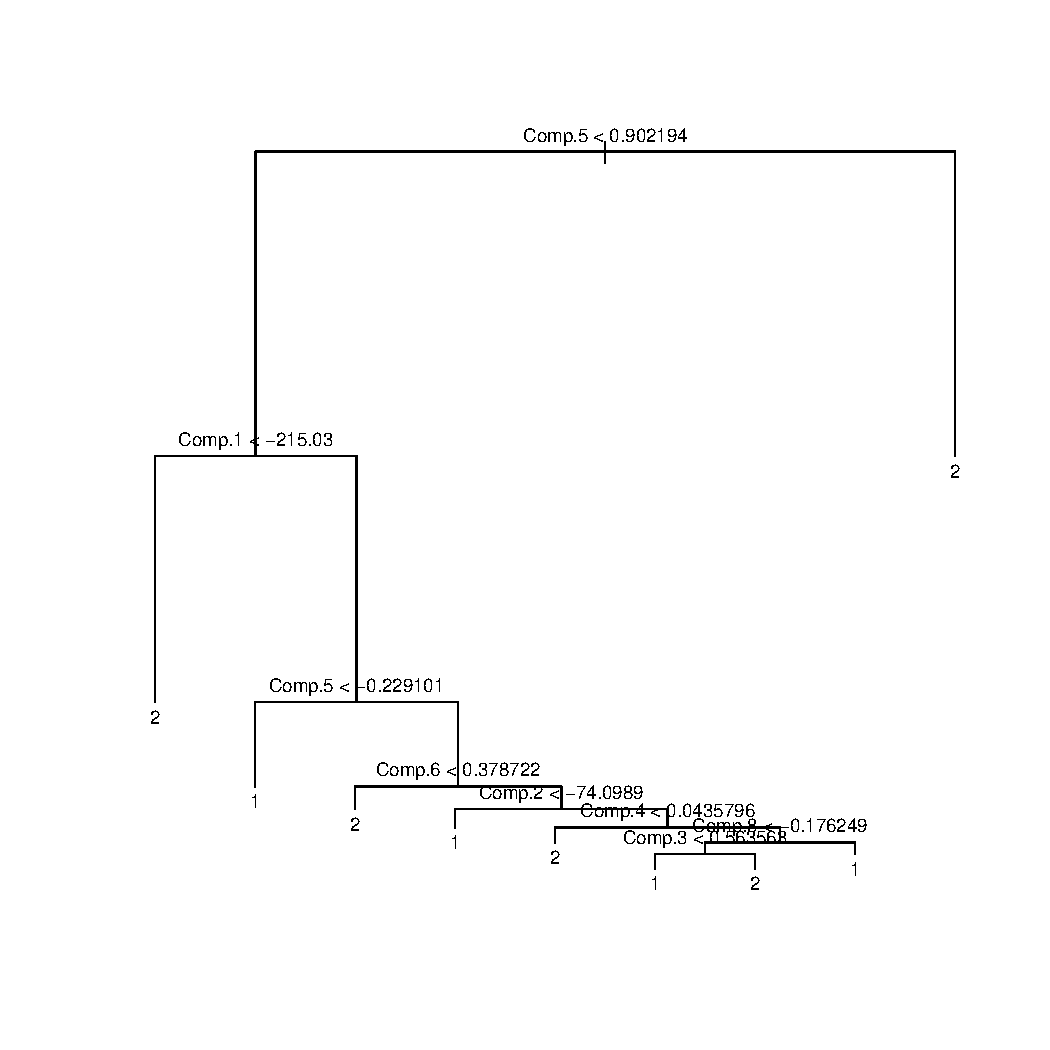
\includegraphics[width=0.35\textwidth]{spam_bin_tree.pdf}
    \captionof{figure}{Arbre de décision obtenue à l'issue d'une séparation aléatoire de $\frac{2}{3}$ du jeu de données \texttt{spam.csv}}
    \label{fig_spam_tree}
\endgroup

\section{Conclusion}
En conclusion, au cours des trois séances de Travaux Pratiques (TP) et de la rédaction du présent rapport, nous avons pu à nouveau prendre conscience de la puissance et des multiples possibilités qui s’offrent à nous en terme de traitement statistique de données avec \texttt{R}. Nous avons également eu l'occasion d'implémenter trois modèles d'analyse discriminante et deux modèles de régression logistique. De plus, nous avons pu tester les performances de ces derniers et des arbres de décision sur différents jeux de données simulées et réelles. Enfin, ce TP nous a permis de mieux comprendre ce qu'était l'apprentissage supervisé.

\newpage
\appendix

% Rajouter toutes les petites fonctions ? Omega1X etc ... ?
\section{Code source Analyse discriminante}
\label{app_sec_code_source_ad}

\subsection{Apprentissage des trois modèles d’analyse discriminante: adq.app, adl.app et nba.app}
\label{app_subsec_app_ad}

\begin{lstlisting}
adq.app <- function(Xapp, zapp){
	g <- max(zapp); # The number of classes
	parameters <- list();
	n <- dim(Xapp)[1];
	for (k in 1:g){
		# K class management
		Xk <- Xapp[which( zapp==k ), ]; # We get the indivuals of this class
		nk <- dim(Xk)[1]; # Number of individuals of this class
		pik <- nk/n; # Proportion of individuals in this class
		muk <- apply(Xk, 2, mean); # Estimation of mu for this class
		sigmak <- cov.wt(Xk, method='ML')$cov; # Estimation of Sigma for this class
		# Here, we store the parameters of the k class
		classK <- list()
		classK$class <- k;
		classK$nk <- nk;
		classK$pik <- pik;
		classK$muk <- muk;
		classK$sigmak <- sigmak;
		parameters[[k]] <- classK;
	}
	parameters;
}
\end{lstlisting}
\begin{lstlisting}
adl.app <- function(Xapp, zapp){
	g <- max(zapp); # The number of classes
	parameters <- list();
	n <- dim(Xapp)[1];
	p <- dim(Xapp)[2];
	sumVk <- matrix(0, nrow=p, ncol=p);
	for (k in 1:g){
		# K class management
		Xk <- Xapp[which( zapp==k ), ]; # We get the indivuals of this class
		nk <- dim(Xk)[1]; # Number of individuals of this classn
		pik <- nk/n; # Proportion of individuals in this class
		muk <- apply(Xk, 2, mean); # Estimation of mu for this class
		sumVk <- sumVk + (nk - 1) * cov.wt(Xk, method='unbiased')$cov;
		# Here, we store the parameters of the k class
		classK <- list()
		classK$class <- k;
		classK$nk <- nk;
		classK$pik <- pik;
		classK$muk <- muk;
		parameters[[k]] <- classK;
	}
	sigmaEstimator <- sumVk/(n-g);
	for (k in 1:g){
		parameters[[k]]$sigmak <- sigmaEstimator;
	}
	parameters;
}
\end{lstlisting}
\begin{lstlisting}
nba.app <- function(Xapp, zapp){
	g <- max(zapp); # The number of classes
	parameters <- list();
	n <- dim(Xapp)[1];
	for (k in 1:g){
		# K class management
		Xk <- Xapp[which( zapp==k ), ]; # We get the indivuals of this class
		nk <- dim(Xk)[1]; # Number of individuals of this class
		pik <- nk/n; # Proportion of individuals in this class
		muk <- apply(Xk, 2, mean); # Estimation of mu for this class
		sigmak <- diag(diag(cov.wt(Xk, method='ML')$cov)); # Estimation of Sigma for this class
		# Here, we store the parameters of the k class
		classK <- list()
		classK$class <- k;
		classK$nk <- nk;
		classK$pik <- pik;
		classK$muk <- muk;
		classK$sigmak <- sigmak;
		parameters[[k]] <- classK;
	}
	parameters;
}
\end{lstlisting}

\subsection{Calcul des probabilités a posteriori : ad.val}
\label{app_subsec_ad_probabilites_a_posteriori}

\begin{lstlisting}
ad.val <- function(parameters, Xtst){
	n <- dim(Xtst)[1];
	g <- length(parameters);
	densities <- list();
	sumDensities <- rep(0, n);
	aPosterioriProbabilities <- NULL;
	for(k in 1:g){
		densities[[k]] <- mvdnorm(Xtst, parameters[[k]]$muk, parameters[[k]]$sigmak);
		sumDensities <- sumDensities + parameters[[k]]$pik * densities[[k]];
	}
	for(k in 1:g){
		if(k == 1){
			aPosterioriProbabilities <- as.matrix((parameters[[k]]$pik * densities[[k]])/sumDensities);
		}else{
			aPosterioriProbabilities <- cbind(aPosterioriProbabilities, as.matrix((parameters[[k]]$pik * densities[[k]])/sumDensities));
		}
	}
	predictions <- apply(aPosterioriProbabilities, 1, which.max);
	predictionsList <- list();
	predictionsList$prob <- aPosterioriProbabilities;
	predictionsList$predictions <- predictions;
	predictionsList;
}
\end{lstlisting}

\section{Code source Régression logistique}
\label{app_sec_reg_log}

\subsection{Apprentissage : log.app}
\label{app_subsec_reg_log_app}

\begin{lstlisting}
log.app  <- function(Xapp, zapp, intr, epsi, pseudoInv=FALSE){
	beta <- NULL; # Estimation of parameters
	niter <- 0; # Number of iterations
	logL <- NULL; # Log vraisemblance
	Xapp <- as.matrix(Xapp);
	n <- dim(Xapp)[1]; # Number of individuals
	p <- dim(Xapp)[2]; # Number of caracteristics
	t <- cleanZ(zapp);	
	minusH <- NULL;
	betaNew <- matrix(0, p, 1);
	betaOld <- matrix(1, p, 1);
	if(intr){ # We should add an intercept
		Xapp <-cbind(matrix(1, n, 1), Xapp);
		betaOld <- matrix(1, p+1, 1);
		betaNew <- matrix(0, p+1, 1);
	}	
	while(norm(betaNew - betaOld, type="2") > epsi){
		niter <- niter + 1;
		betaOld <- betaNew;
		minusH <- t(Xapp) %*% diag( diag( pOmega1X(Xapp, betaOld) %*% t(pOmega2X(Xapp, betaOld)) ) )  %*% Xapp;
		if(pseudoInv){
			betaNew <- betaOld + ginv(minusH) %*% t(Xapp) %*% (t - pOmega1X(Xapp, betaOld));
		}else{
			betaNew <- betaOld + solve(minusH) %*% t(Xapp) %*% (t - pOmega1X(Xapp, betaOld));
		}	
	}
	results <- list()
	results$beta <- betaNew;
	results$niter <- niter;
	results$logL <- t(Xapp) %*% (t - pOmega1X(Xapp, betaNew));
	results;
}
\end{lstlisting}

\subsection{Classement : log.val}
\label{app_subsec_reg_log_val}

\begin{lstlisting}
log.val <- function(beta, Xtst){
	Xtst <- as.matrix(Xtst);
	n <- dim(Xtst)[1];
	p <- dim(Xtst)[2];
	pBeta <- dim(beta)[1];
	if(p != pBeta){ 
		Xtst <-cbind(matrix(1, n, 1), Xtst);
	}
 	results <- list();
 	prob <- post.pr(Xtst, beta);
 	predictions <- apply(prob, 1, which.max);
 	results$prob <- prob;
 	results$predictions <- predictions;
 	results;
}
\end{lstlisting}

\subsection{Régression logistique quadratique : log.quad.app et  log.quad.val}
\label{app_subsec_reg_log_val_app_quad}

\begin{lstlisting}
log.quad.app  <- function(Xapp, zapp, epsi, pseudoInv=FALSE){
	Xapp <- as.matrix(Xapp);
	Xapp <- computeQuadraticModel(Xapp);
	log.app(Xapp, zapp, FALSE, epsi, pseudoInv);
}

computeQuadraticModel <- function(X){
	n <- dim(X)[1];
	p <- dim(X)[2];
	XNew <- matrix(0, n, (p*(p+1))/2);
	iterator <- 0;
	for(i in 1:(p-1)){
		for(j in (i+1):p){
			iterator <- iterator + 1;
			XNew[, iterator] <- X[, i] * X[, j]; 
		}
	}
	for(i in 1:p){
		iterator <- iterator + 1;
		XNew[, iterator] <- X[, i] * X[, i]; 
	}
 	cbind(X, XNew);
}
\end{lstlisting}

\end{multicols}
\end{document}